\documentclass[conference]{IEEEtran}
\IEEEoverridecommandlockouts

\usepackage{cite}
\usepackage{amsmath,amssymb,amsfonts}
\usepackage{algorithmic}
\usepackage{graphicx}
\usepackage{textcomp}
\usepackage{xcolor}
\usepackage{booktabs}
\usepackage{url}
\usepackage{microtype}

\def\BibTeX{{\rm B\kern-.05em{\sc i\kern-.025em b}\kern-.08em
    T\kern-.1667em\lower.7ex\hbox{E}\kern-.125emX}}

\begin{document}

\title{MonsoonIQ: Hyperlocal Monsoon Onset Dynamics and Regime-Aware Agricultural Advisory Intelligence for Maharashtra, India}

\author{\IEEEauthorblockN{Ashwell Cherian Giji}
\IEEEauthorblockA{\textit{School of AI and ML and Emerging Technologies} \\
\textit{Lovely Professional University}\\
Phagwara, Punjab, India \\
ashwellcheriangiji@gmail.com}
\and
\IEEEauthorblockN{Apoorv Dubey}
\IEEEauthorblockA{\textit{Department of Computer Science and Engineering,} \\
\textit{School of Computer Science and Engineering}\\
\textit{Lovely Professional University}\\
Phagwara, Punjab, India \\
apoorvdubey@gmail.com}
}

\maketitle

\begin{abstract}
In rainfed tropical agriculture, determining the optimal Kharif sowing window is critical to preventing crop failure. In Maharashtra, India, official India Meteorological Department (IMD) monsoon declarations operate at macro-subdivision scales, obscuring extreme orographic and agro-climatic gradients. Farmers adopting simplistic rainfall accumulation thresholds (e.g., sowing after 50~mm of rain) frequently incur severe seedling desiccation when early showers are followed by prolonged dry spells. This paper presents \textit{MonsoonIQ}, an end-to-end computational framework that transforms 23 years (2001--2023) of high-resolution ($0.25^\circ \times 0.25^\circ$) IMD gridded daily rainfall data across 419 valid onshore grid cells (9,637 cell-years) into actionable agricultural intelligence. We propose an objective two-stage Local Sustained Onset Detection Algorithm that filters pre-monsoon convective bursts from genuine monsoonal progression, confirming 9,606 onset events (99.68\% detection rate). Using nine engineered onset-dynamics features, unsupervised machine learning ($K$-Means, $K=4$) identifies four distinct agro-climatic regimes: Core Interior Synchronized (51.31\%), Interior Semi-Arid Transition (23.15\%), Early Maritime \& Western Ghats (15.51\%), and Rain-Shadow High-Volatility (10.02\%). Clustering robustness is validated via Silhouette Analysis (0.2987), Davies-Bouldin Index (1.1948), cross-algorithm agreement with Agglomerative Hierarchical clustering (87.83\% agreement, $\text{ARI}=0.6803$), and spatial autocorrelation (Moran's $I > 0.50$, contiguity 75.30\%). Crucially, we uncover the ``Rain-Shadow Anomaly'', wherein arid rain-shadow cells satisfy a 50~mm trigger 4--7 days earlier than wetter zones due to convective bursts, yet 39.13\% of these trigger events are followed by catastrophic $\ge 10$-day dry breaks. To mitigate this hazard, MonsoonIQ implements a regime-aware advisory state machine enforcing an audited 75~mm threshold, a multi-day persistence requirement, and an active wetting-cycle reset mechanism that discounts evaporated moisture following $\ge 10$-day dry spells. Evaluated across historical and simulated scenarios without promising deceptive ``safe to sow'' guarantees, MonsoonIQ demonstrates how unsupervised machine learning and empirical agrometeorology bridge the gap between raw climate grids and farm-level risk management.
\end{abstract}

\begin{IEEEkeywords}
Monsoon Onset Detection, Rainfall Analysis, K-Means Clustering, Agricultural Decision Support, Maharashtra, Geospatial Analytics, Dry Spell Analysis, Climate Intelligence.
\end{IEEEkeywords}

\section{Introduction}
\IEEEPARstart{R}{ainfed} agriculture supports over 60\% of India's cultivated area and underpins the livelihoods of millions of smallholder farmers across the semi-arid tropics~\cite{sivakumar2005impacts}. In the state of Maharashtra, the southwest monsoon (June--September, JJAS) accounts for upwards of 80\% of annual precipitation~\cite{gadgil2003indian}. Timing the commencement of Kharif (monsoon-season) crop sowing is the single most consequential economic decision a dryland farmer makes. Sowing too early risks fatal seedling mortality if initial rains are followed by a prolonged dry spell; sowing too late shortens the vegetative growth window, induces flowering delays, and exposes crops to terminal moisture stress during September grain-filling~\cite{gadgil2000farming,rao2013rainfall}.

Historically, official monsoon onset declarations issued by the India Meteorological Department (IMD) have focused on large-scale synoptic criteria: kinetic energy increases in lower-tropospheric winds (850~hPa), depth of westerlies, and out-going longwave radiation (OLR) thresholds over the southeastern Arabian Sea and Kerala~\cite{ananthakrishnan1988onset,pai2014development}. While vital for macroeconomic and national planning, these regional declarations are fundamentally unsuited for local farm-level operations~\cite{hansen2019climate}. Maharashtra spans a dramatic orographic barrier in the Western Ghats (Sahyadri range), dropping precipitously into an arid rain-shadow plateau before transitioning into the continental black-soil plains of Marathwada and Vidarbha~\cite{gadgil2003indian,wani2003integrated}. Consequently, declaring that the ``monsoon has covered Maharashtra'' offers zero operational guidance to a Vertisol farmer in Solapur experiencing an isolated convective burst compared to a coastal rice farmer in Ratnagiri receiving continuous orographic rain.

In response to regional declarations, public extension services have traditionally recommended generic empirical rules, most notably advising farmers to sow once cumulative seasonal rainfall achieves 50~mm~\cite{crida2020contingency}. However, empirical evidence demonstrates that topsoil wetting in cracking clay soils (Vertisols) requires substantially more moisture under high pre-monsoon evaporative demand ($\text{ET}_0 > 5\text{ mm/day}$)~\cite{allen1998crop,mpkv2022package}. Simplistic 50~mm accumulation counters fail to differentiate between sustained monsoonal inflow and transient pre-monsoon thunderstorms, leading to widespread seed desiccation.

To address these limitations, this paper presents \textbf{MonsoonIQ}, a comprehensive climatological data engineering and machine learning framework. The primary contributions of this work are:
\begin{enumerate}
    \item \textbf{Hyperlocal Climatological Pipeline:} Standardization of 23 years (2001--2023) of IMD $0.25^\circ \times 0.25^\circ$ daily gridded rainfall across 419 valid onshore Maharashtra cells (9,637 cell-years), preserving raw missing values without artificial zero-imputation.
    \item \textbf{Local Sustained Onset Algorithm:} Formulation of a two-stage detection algorithm combining running-window accumulation triggers with post-candidate dry-spell filtering, identifying 9,606 confirmed onsets.
    \item \textbf{Unsupervised Regime Discovery:} Unsupervised clustering ($K$-Means, $K=4$) over nine engineered onset features, identifying four distinct agro-climatic zones validated via cross-algorithm benchmarks, bootstrap resampling, and spatial contiguity metrics.
    \item \textbf{Empirical Resolution of the Rain-Shadow Paradox:} Detailed mathematical investigation of why arid rain-shadow cells hit simplistic 50~mm triggers prematurely, proving that 39.13\% of such triggers encounter fatal $\ge 10$-day breaks.
    \item \textbf{Audited Sowing Advisory Engine:} Implementation of a transparent four-state decision machine incorporating active wetting-cycle resets and strict prohibition of misleading ``safe to sow'' guarantees.
\end{enumerate}

\section{Related Work}
\subsection{Monsoon Onset Climatology and Local Detection}
The onset of the southwest monsoon has been investigated extensively at the continental scale. Ananthakrishnan and Soman~\cite{ananthakrishnan1988onset} established the foundational statistical definition of onset over Kerala based on sharp transitions in 5-day daily rainfall averages. Soman and Kumar~\cite{soman1993space} and Joseph et al.~\cite{joseph1994interannual} analyzed the synoptic-scale circulation features accompanying onset transitions across peninsular India. Rajeevan et al.~\cite{ra जीवन2006high} and Pai et al.~\cite{pai2014development} developed the high-resolution ($0.25^\circ \times 0.25^\circ$) daily gridded rainfall datasets that enabled localized spatial analysis. However, translating synoptic onset into localized agronomic criteria remains challenging; localized definitions must distinguish between transient convective pre-monsoon showers and sustained monsoonal westerlies~\cite{gadgil2003indian}.

\subsection{Rainfall Variability and Dry Spells in Maharashtra}
Rainfall variability in peninsular India is strongly modulated by the Western Ghats orography. Rao et al.~\cite{rao2013rainfall} analyzed dry spells in the rain-shadow districts of Maharashtra (Solapur, Ahmednagar), demonstrating that early Kharif dry spells exceeding 10 days occur in over 70\% of seasons. Wani et al.~\cite{wani2003integrated} investigated soil-water balance in semi-arid Vertisols, emphasizing that cracking black soils exhibit high water-holding capacities but require deep wetting pulses ($\ge 75\text{ mm}$) to support seedling emergence without surface crusting. Institutional guidelines from ICAR-CRIDA~\cite{crida2020contingency} and MPKV Rahuri~\cite{mpkv2022package} highlight the necessity of contingency planning when sowing is delayed past July 15.

\subsection{Machine Learning and Climate Regime Discovery}
Unsupervised clustering techniques have been widely applied to climate time series for regionalization. MacQueen's $K$-Means algorithm~\cite{macqueen1967some} remains the benchmark for climatological partitioning due to its computational scalability and spherical variance minimization. Cluster validation frameworks proposed by Rousseeuw (Silhouette Analysis)~\cite{rousseeuw1987silhouettes}, Davies and Bouldin~\cite{davies1979cluster}, and Cali{\'n}ski and Harabasz~\cite{calinski1974dendrite} provide quantitative criteria for selecting cluster numbers. Spatial autocorrelation measures, notably Moran's $I$~\cite{moran1950notes}, verify that statistical clusters exhibit physical spatial coherence. In agro-meteorology, Stone and Meinke~\cite{stone2005operational} and Hansen et al.~\cite{hansen2019climate} emphasized that climate advisory systems must communicate uncertainty transparently rather than delivering deterministic guarantees.

\begin{figure}[t]
\centering
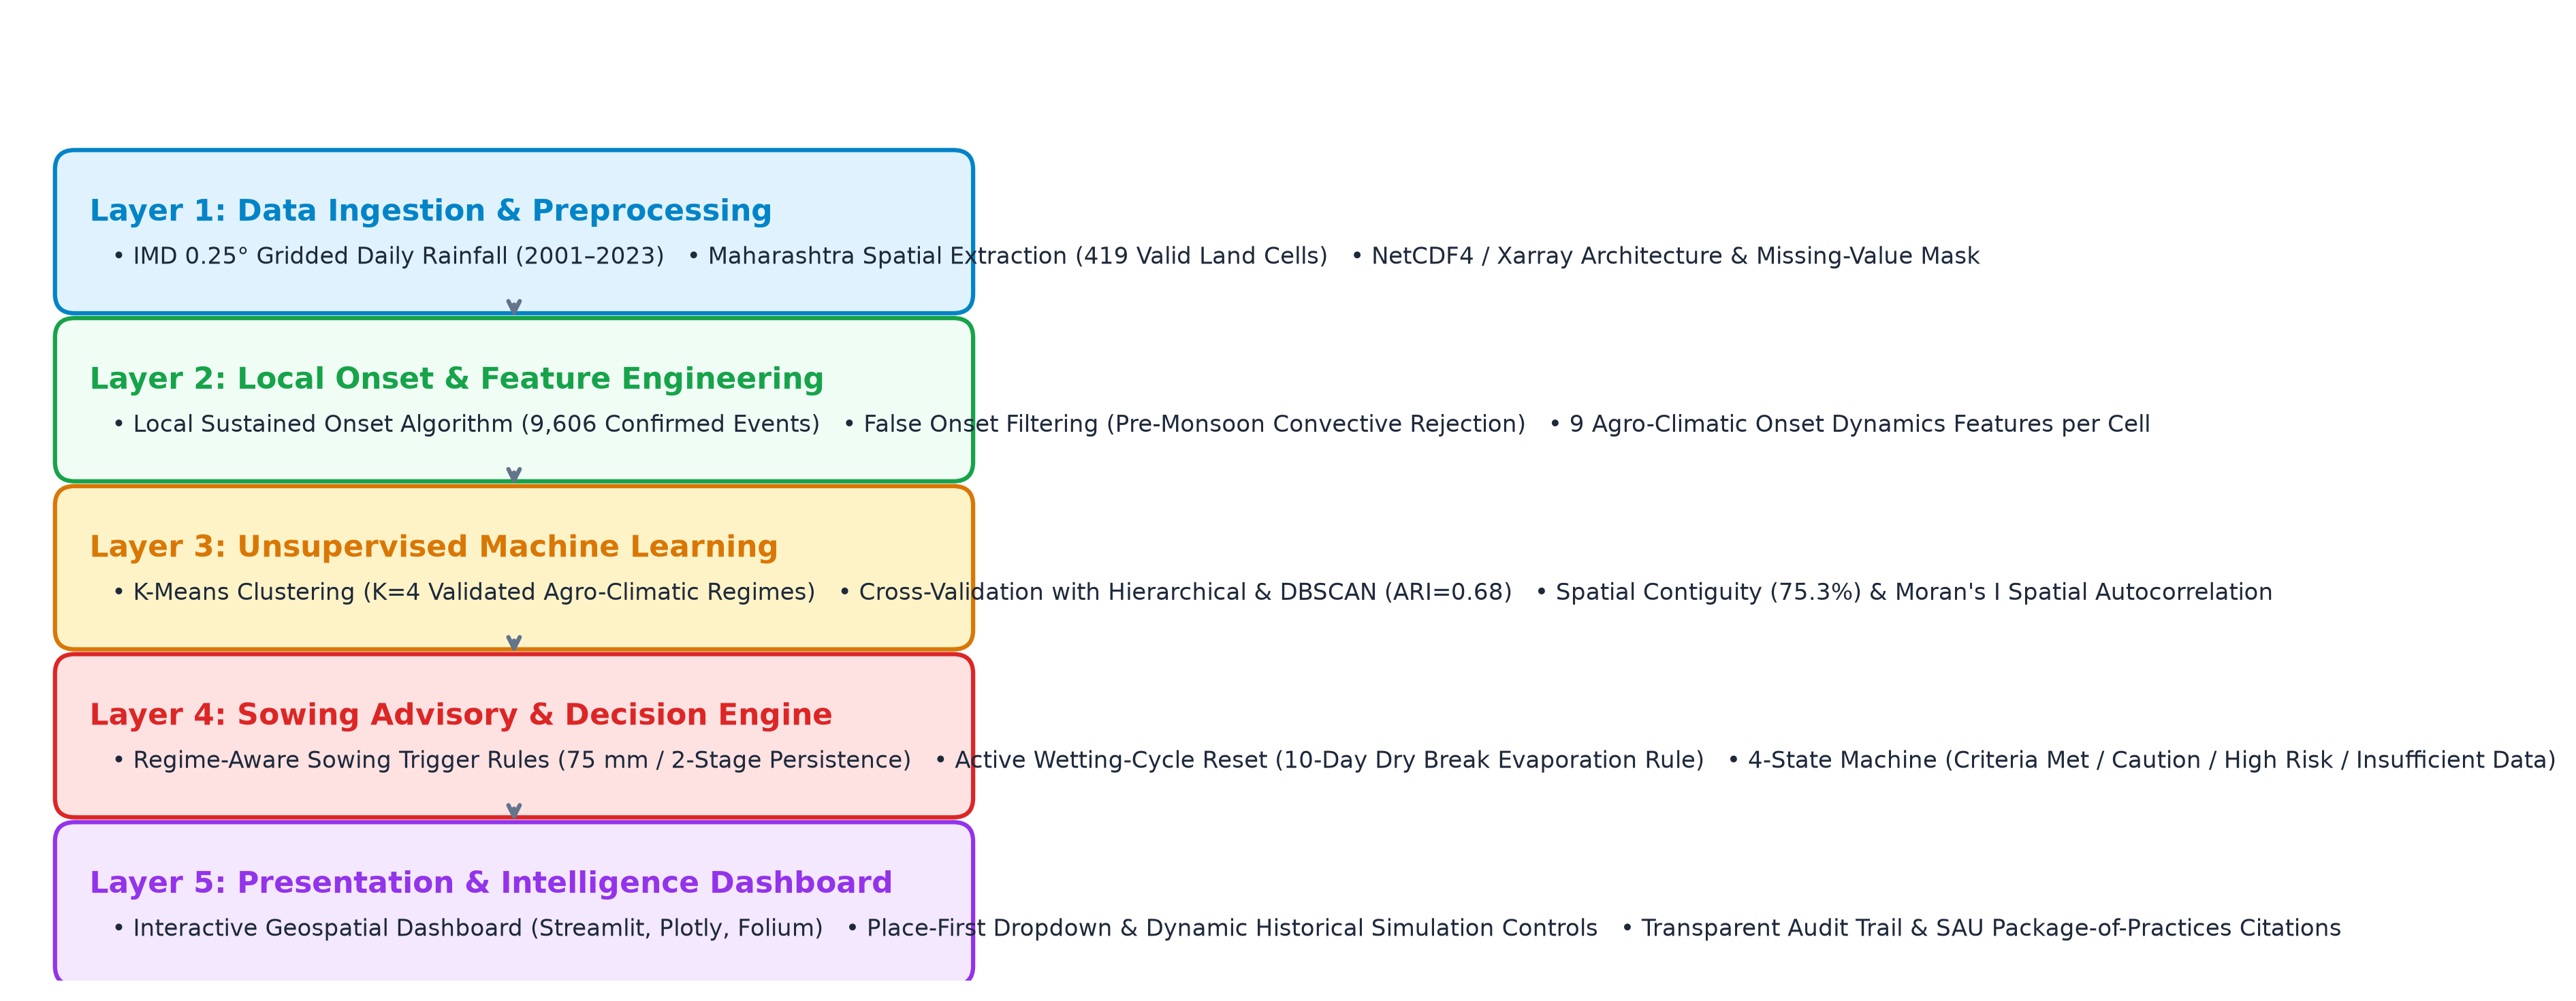
\includegraphics[width=\columnwidth]{figures/fig_system_architecture.png}
\caption{MonsoonIQ overall system architecture spanning data ingestion, local onset detection, unsupervised ML clustering, decision logic, and presentation layers.}
\label{fig:architecture}
\end{figure}

\section{Study Area and Dataset}
\subsection{Geographical and Climatic Profile of Maharashtra}
Maharashtra covers an area of 307,713~$\text{km}^2$ in western and central India ($15.75^\circ\text{N}$--$22.00^\circ\text{N}$, $72.75^\circ\text{E}$--$80.75^\circ\text{E}$). The state exhibits three physiographic provinces:
\begin{enumerate}
    \item \textbf{The Konkan Coastal Lowlands:} A narrow strip bounded by the Arabian Sea and the Western Ghats, receiving intense orographic precipitation ($>2,800\text{ mm}$ annually).
    \item \textbf{The Western Ghats (Sahyadri):} A continuous escarpment rising to 1,200--1,600~m, inducing extreme leeward precipitation dissipation.
    \item \textbf{The Deccan Plateau:} Comprising the arid Rain-Shadow belt (Solapur, Ahmednagar), the Marathwada semi-arid transition zone, and the eastern Vidarbha plains.
\end{enumerate}

\subsection{IMD High-Resolution Gridded Dataset}
This research utilizes the India Meteorological Department (IMD) $0.25^\circ \times 0.25^\circ$ daily gridded rainfall product~\cite{pai2014development}. The dataset interpolates observations from over 6,500 surface rain-gauge stations across India using the Shepard local-weighting interpolation scheme:
\begin{itemize}
    \item \textbf{Spatial Domain:} Bounding box of 28 latitudes $\times$ 35 longitudes (980 total grid cells).
    \item \textbf{Masking:} Spatial masking against official Survey of India boundary vectors yields exactly \textbf{419 valid onshore land cells} inside Maharashtra (50 marine cells and 511 non-Maharashtra terrestrial cells excluded).
    \item \textbf{Temporal Span:} 23 consecutive years from January 1, 2001 to December 31, 2023 (8,400 consecutive calendar days per grid cell).
    \item \textbf{Data Volume:} $419 \times 8,400 = 3,519,600$ terrestrial daily observations. NetCDF4 storage size is 14.35~MB.
    \item \textbf{Missing-Data Preservation:} Terrestrial observations maintain 0.0\% missing values. Marine cells are encoded strictly as IEEE \texttt{NaN}. No artificial zero-filling or synthetic smoothing is applied.
\end{itemize}

\begin{figure}[t]
\centering
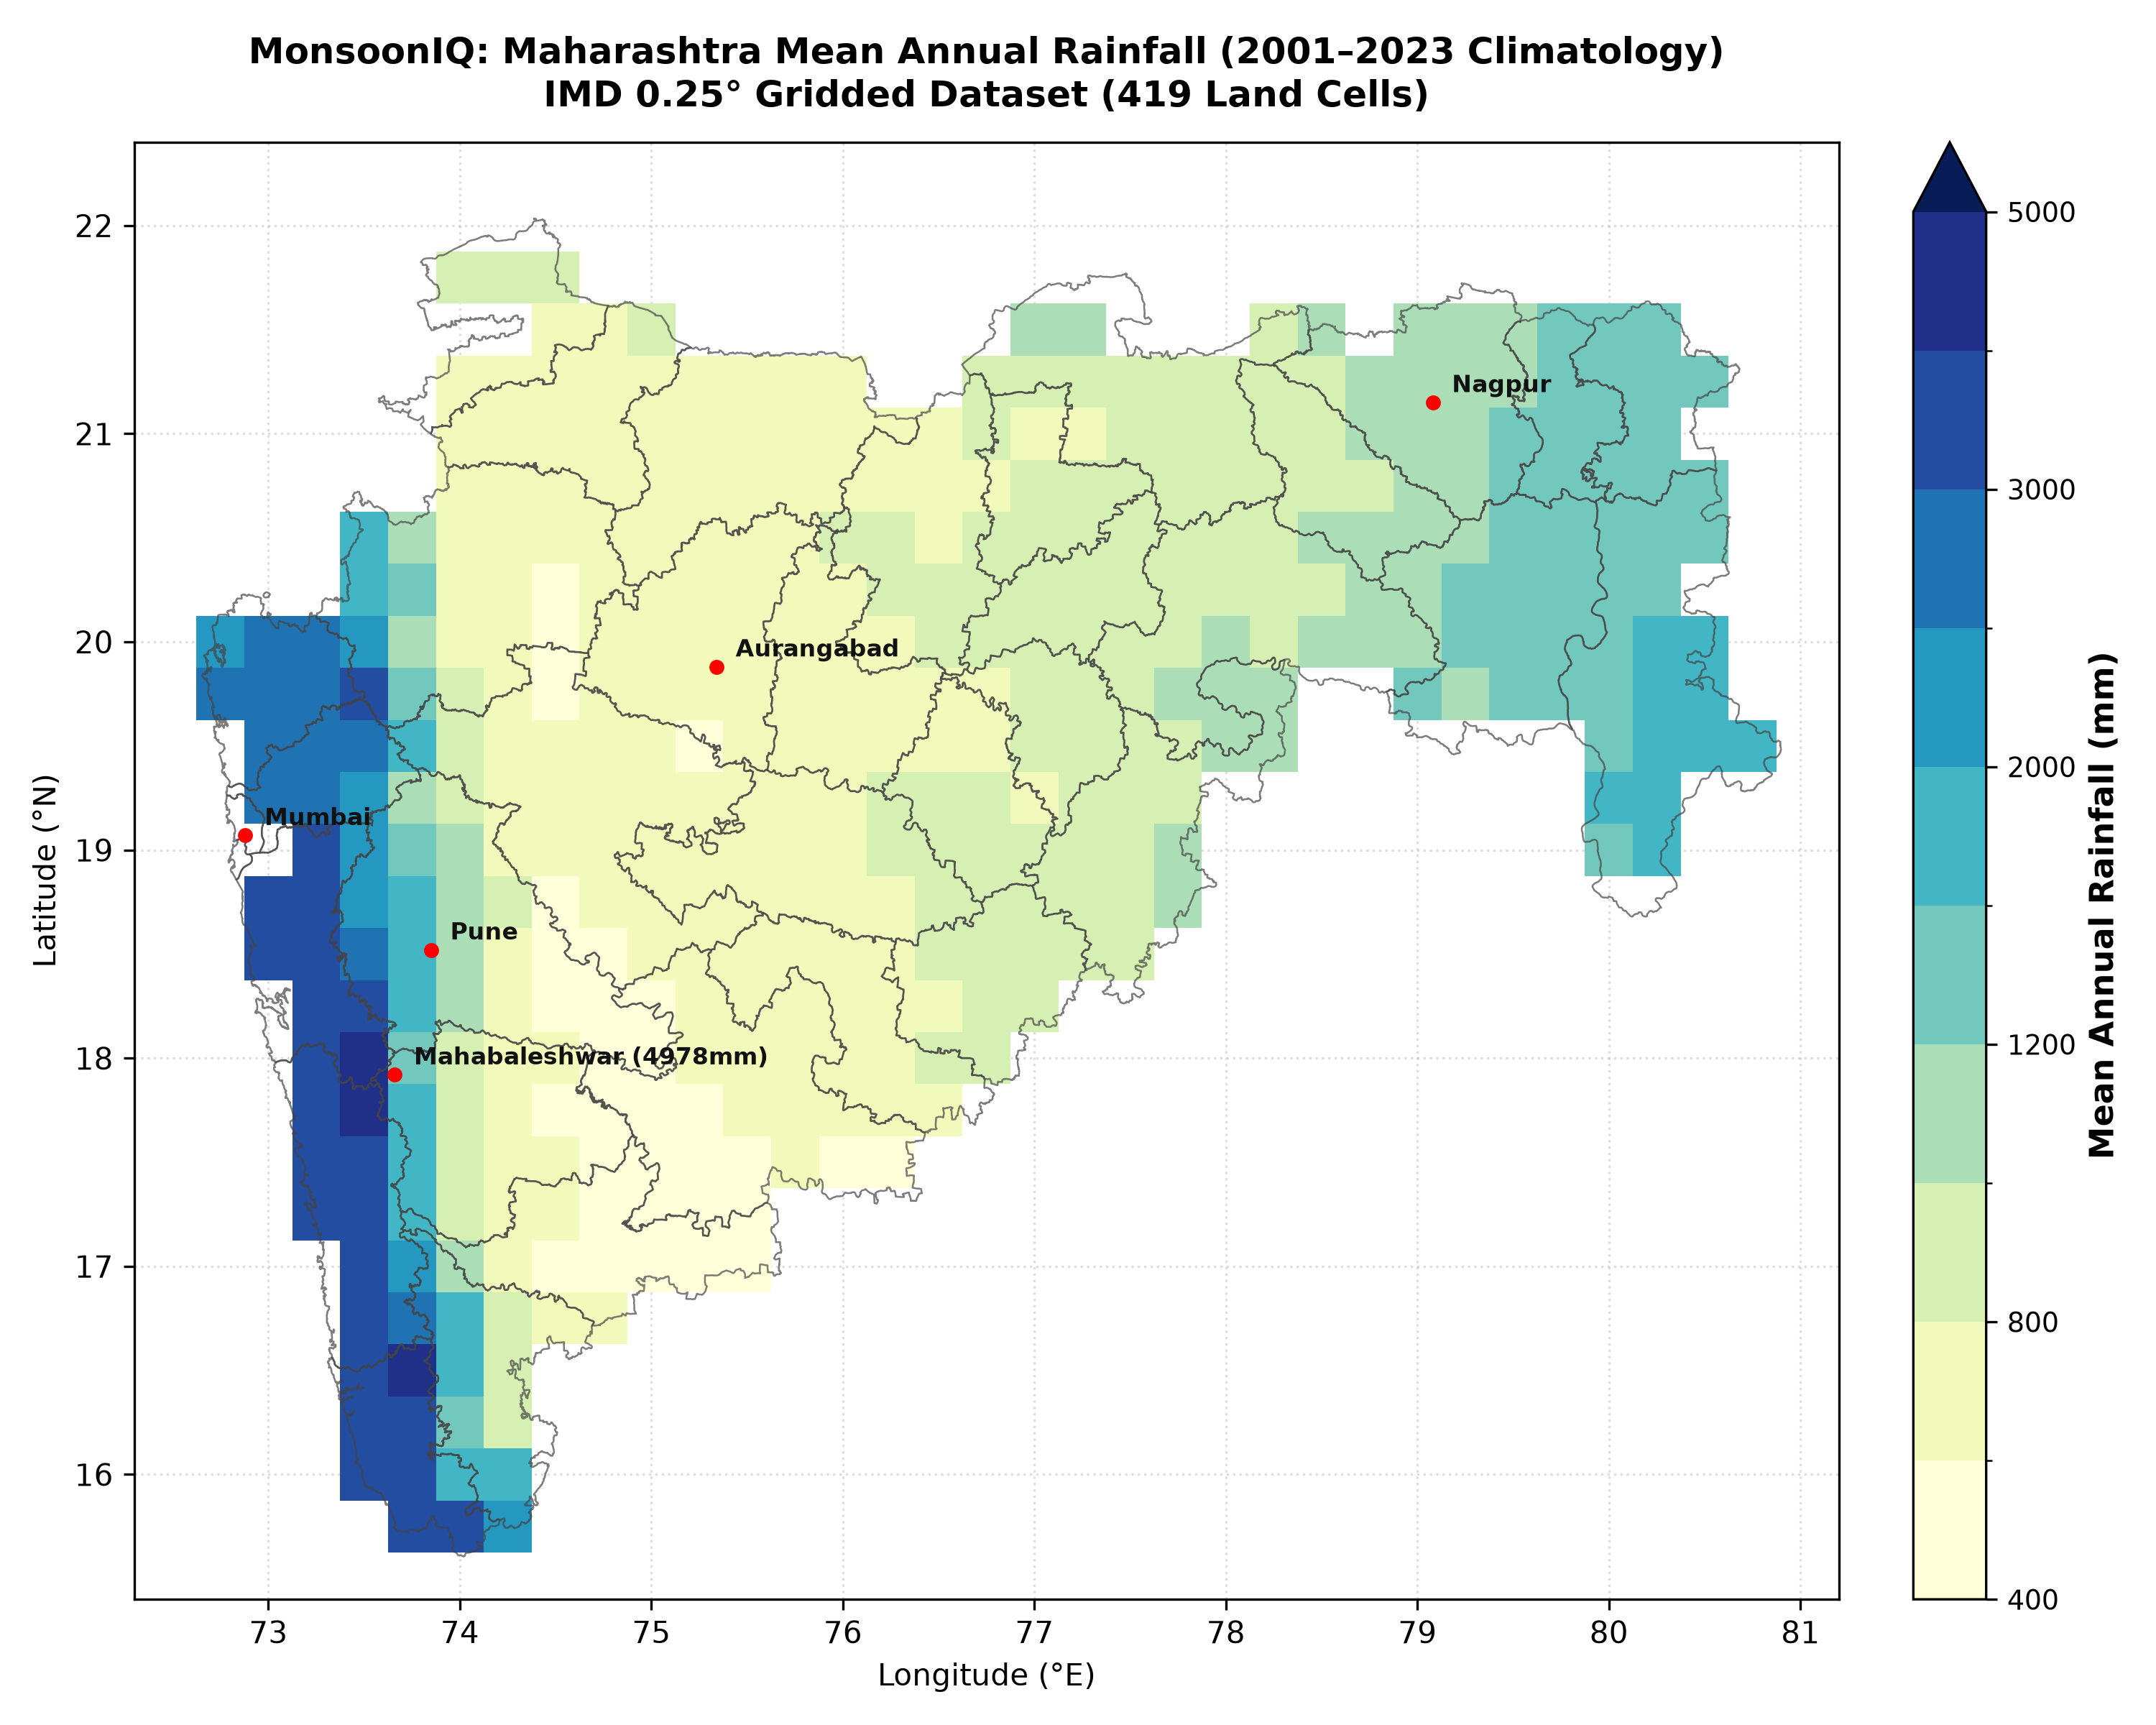
\includegraphics[width=\columnwidth]{figures/fig_annual_rainfall.png}
\caption{Spatial distribution of climatological mean annual rainfall across Maharashtra (2001--2023), highlighting the Western Ghats orographic gradient.}
\label{fig:annual_rainfall}
\end{figure}

\begin{figure}[t]
\centering
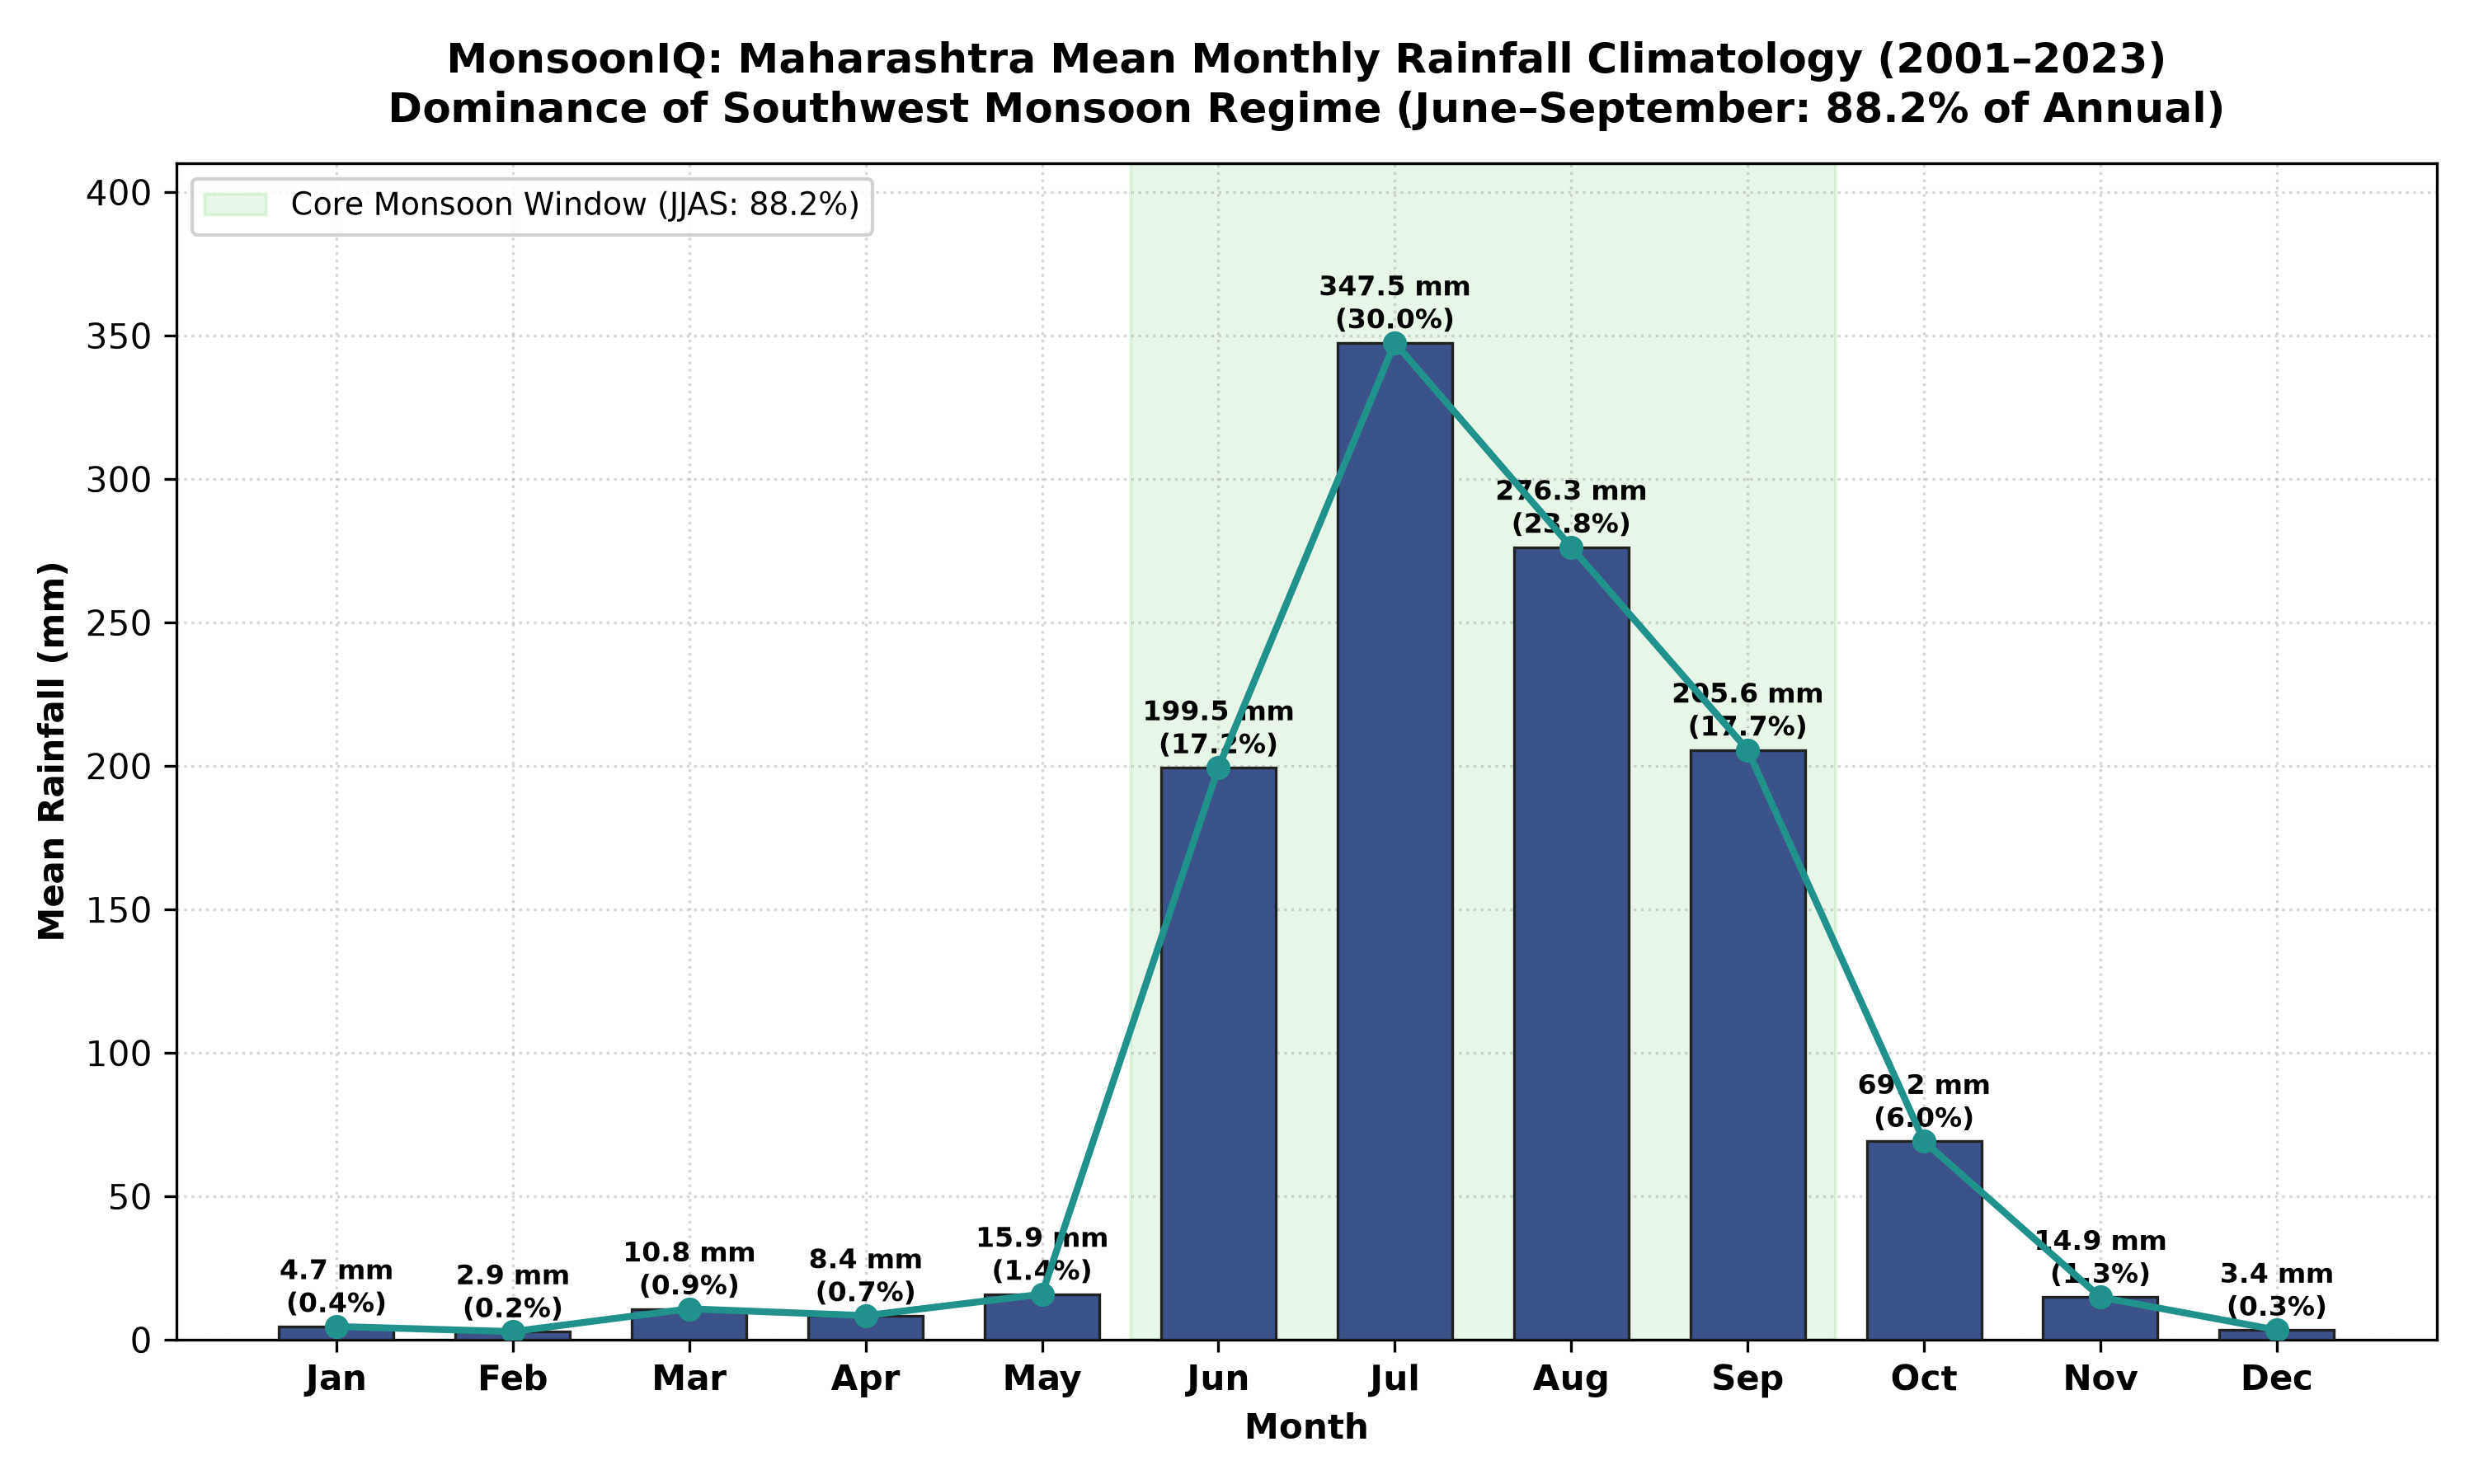
\includegraphics[width=\columnwidth]{figures/fig_monthly_climatology.png}
\caption{Climatological monthly rainfall distribution across meteorological subdivisions, highlighting rainfall concentration in July and August.}
\label{fig:monthly_climatology}
\end{figure}

\section{Proposed Methodology}
The MonsoonIQ methodology comprises five computational modules: local sustained onset detection, feature engineering, unsupervised clustering, sowing trigger sensitivity auditing, and the regime-aware advisory state machine.

\subsection{Local Sustained Onset Detection Algorithm}
Let $R_{c,y}(t)$ denote daily rainfall (in mm) at grid cell $c$ on day-of-year $t \in [1, 365]$ in year $y$. The algorithm initiates monitoring on June 1 ($t = 152$, non-leap year) following a pre-monsoon buffer starting May 15 ($t = 135$).

\subsubsection{Candidate Trigger Identification}
A candidate onset date $t^* \in [152, 212]$ (June 1 to July 31) is triggered on the first day satisfying a multi-day accumulation pulse:
\begin{equation}
\sum_{k=0}^{W-1} R_{c,y}(t - k) \ge \Theta_{\mathrm{pulse}} \quad \text{and} \quad R_{c,y}(t) \ge R_{\mathrm{wet}}
\label{eq:pulse}
\end{equation}
where $W = 5$ days, $\Theta_{\mathrm{pulse}} = 25.0\text{ mm}$, and $R_{\mathrm{wet}} = 2.5\text{ mm}$ (IMD rainy day threshold).

\subsubsection{False Onset Filtering}
To reject transient pre-monsoon convective thunderstorms, candidate $t^*$ is evaluated over a subsequent verification window $V = 15$ days:
\begin{equation}
L_{\mathrm{dry}}(t^*) = \max_{t^* < \tau \le t^* + V} \left\{ \sum_{i=0}^{d-1} \mathbb{I}(R_{c,y}(\tau + i) < R_{\mathrm{wet}}) \right\}
\label{eq:dry_spell}
\end{equation}
where $\mathbb{I}(\cdot)$ is the indicator function. The candidate is classified as a \textit{false onset} and rejected if:
\begin{equation}
L_{\mathrm{dry}}(t^*) \ge L_{\mathrm{crit}} \quad (L_{\mathrm{crit}} = 10\text{ days})
\end{equation}
If rejected, the search advances to $t^* + 1$. If $L_{\mathrm{dry}}(t^*) < L_{\mathrm{crit}}$, $t^*$ is confirmed as the \textit{Local Sustained Onset Date} $D_{c,y}$. If no date satisfies the criteria by July 31 ($t=212$), the season is recorded as a non-detection event ($D_{c,y} = \text{NaN}$).

\begin{figure}[t]
\centering
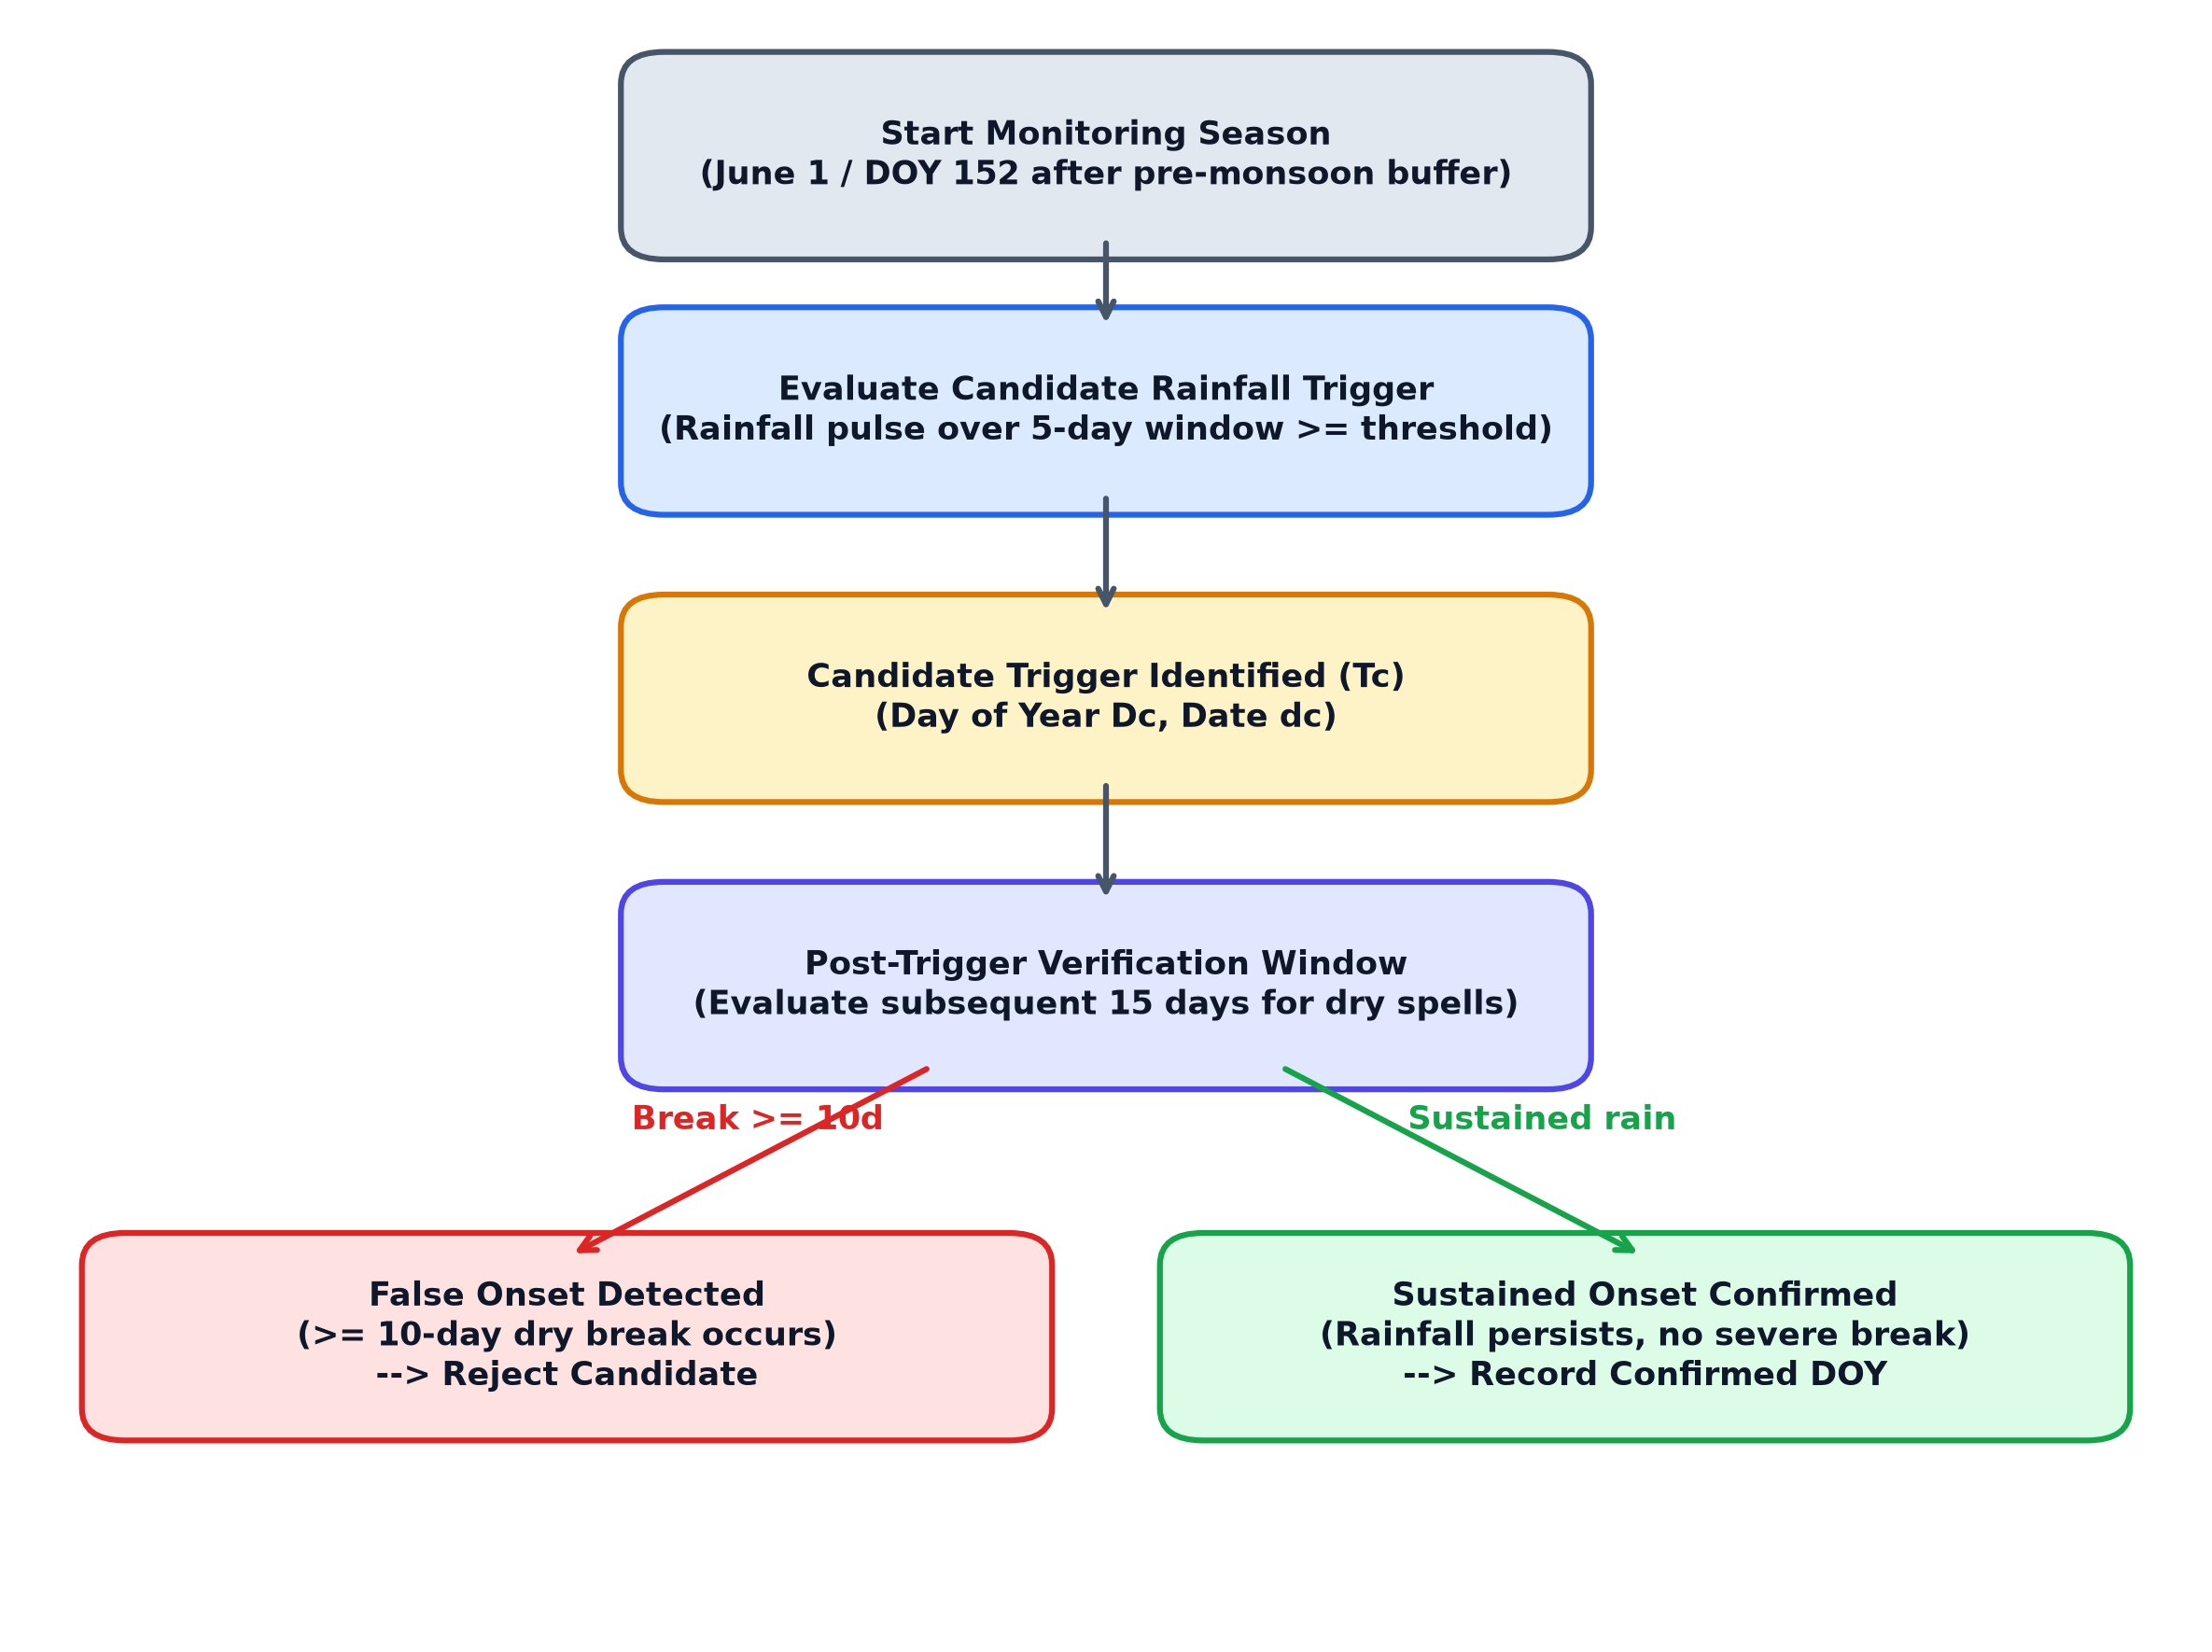
\includegraphics[width=0.9\columnwidth]{figures/fig_onset_detection_workflow.png}
\caption{Flowchart of the two-stage Local Sustained Onset Detection Algorithm, separating sustained monsoonal progression from transient convective bursts.}
\label{fig:onset_workflow}
\end{figure}

\subsection{Agro-Climatic Feature Engineering}
To capture multidimensional onset dynamics, each grid cell $c$ is mapped to a 9-dimensional feature vector $\mathbf{x}_c \in \mathbb{R}^9$ computed across the 23-year historical record:
\begin{enumerate}
    \item \textbf{Median Onset DOY ($\tilde{D}_c$):} Median confirmed onset day of year.
    \item \textbf{Mean Onset DOY ($\bar{D}_c$):} Arithmetic mean onset day of year.
    \item \textbf{Onset Std. Dev. ($\sigma_{D,c}$):} Interannual temporal variability:
    \begin{equation}
    \sigma_{D,c} = \sqrt{\frac{1}{N_{y}-1}\sum_{y=1}^{N_y} (D_{c,y} - \bar{D}_c)^2}
    \end{equation}
    \item \textbf{Interquartile Range ($\text{IQR}_c$):} Spread between 75th and 25th percentiles: $Q_3(D_c) - Q_1(D_c)$.
    \item \textbf{Early Onset Frequency ($f_{\mathrm{early},c}$):} Fraction of years with $D_{c,y} \le 156$ (June 5).
    \item \textbf{Delayed Onset Frequency ($f_{\mathrm{delayed},c}$):} Fraction of years with $D_{c,y} \ge 176$ (June 25).
    \item \textbf{Candidate Rejection Frequency ($f_{\mathrm{reject},c}$):} Mean annual rate of false onset candidate rejections:
    \begin{equation}
    f_{\mathrm{reject},c} = \frac{1}{N_y} \sum_{y=1}^{N_y} N_{\mathrm{rejected},c,y}
    \end{equation}
    \item \textbf{Mean Max Early Dry Spell ($\bar{L}_{\mathrm{dry},c}$):} Climatological mean length of the maximum consecutive dry spell in June.
    \item \textbf{Onset Detection Frequency ($f_{\mathrm{det},c}$):} Proportion of years with a confirmed onset event: $f_{\mathrm{det},c} = \frac{1}{N_y}\sum_{y=1}^{N_y} \mathbb{I}(D_{c,y} \neq \text{NaN})$.
\end{enumerate}

\subsection{Unsupervised Clustering and Validation Metrics}
Feature matrix $\mathbf{X} \in \mathbb{R}^{419 \times 9}$ is standardized using $z$-score normalization: $\mathbf{Z} = (\mathbf{X} - \boldsymbol{\mu}) / \boldsymbol{\sigma}$.

\subsubsection{K-Means Clustering}
$K$-Means partitions the 419 cells into $K$ disjoint clusters $\mathcal{C} = \{C_1, \dots, C_K\}$ by minimizing within-cluster sum of squares (WCSS):
\begin{equation}
J = \sum_{k=1}^K \sum_{\mathbf{z}_i \in C_k} \|\mathbf{z}_i - \mathbf{m}_k\|^2
\label{eq:kmeans}
\end{equation}
where $\mathbf{m}_k = \frac{1}{|C_k|}\sum_{\mathbf{z}_i \in C_k} \mathbf{z}_i$. We execute $K$-Means with $K=4$, $n_{\mathrm{init}} = 50$, and maximum iterations $= 300$.

\subsubsection{Validation Metrics}
Cluster quality is quantitatively assessed using:
\begin{itemize}
    \item \textbf{Silhouette Coefficient ($S$):} For cell $i$, $s(i) = \frac{b(i) - a(i)}{\max(a(i), b(i))}$, where $a(i)$ is mean intra-cluster distance and $b(i)$ is minimum mean inter-cluster distance.
    \item \textbf{Davies-Bouldin Index ($DB$):} Average similarity ratio between each cluster and its most similar counterpart:
    \begin{equation}
    DB = \frac{1}{K} \sum_{i=1}^K \max_{j \neq i} \left\{ \frac{s_i + s_j}{d(\mathbf{m}_i, \mathbf{m}_j)} \right\}
    \end{equation}
    \item \textbf{Cali{\'n}ski-Harabasz Index ($CH$):} Ratio of between-cluster dispersion to within-cluster dispersion.
    \item \textbf{Adjusted Rand Index (ARI):} Compares cluster partition stability against alternative clustering algorithms (Agglomerative Hierarchical, Ward linkage) and bootstrap subsampling~\cite{hubert1985comparing}.
\end{itemize}

\subsection{Sowing Advisory Decision Engine & Accumulation Semantics}
The advisory engine operates as a deterministic finite-state machine evaluating daily rainfall vectors $\mathbf{R}_{c,y}$ up to date $t_{\mathrm{as\_of}}$.

\subsubsection{Active Wetting-Cycle Reset Rule}
In semi-arid Vertisols, high pre-monsoon potential evapotranspiration ($\text{ET}_0 > 5\text{ mm/day}$) rapidly desiccates topsoil moisture~\cite{allen1998crop}. When an intervening dry break $\Delta t_{\mathrm{dry}} \ge 10$ consecutive days occurs between early rain and recent showers, moisture from earlier rain is treated as fully evaporated. The effective cumulative rainfall counter $R_{\mathrm{eff}}$ resets:
\begin{equation}
R_{\mathrm{eff}}(t) = 
\begin{cases} 
0.0\text{ mm}, & \text{if } L_{\mathrm{consec\_dry}}(t) \ge 10 \\
\sum_{\tau = t_{\mathrm{reset}}}^t R_{c,y}(\tau), & \text{otherwise}
\end{cases}
\label{eq:reset}
\end{equation}
where $t_{\mathrm{reset}}$ marks the resumption of rainfall following the break.

\subsubsection{Advisory State Logic}
The engine evaluates four distinct states:
\begin{enumerate}
    \item \textbf{INSUFFICIENT DATA (Gray):} Triggered if data completeness is $<80\%$ or if missing observations occur within the 5-day verification window.
    \item \textbf{CAUTION (Yellow):} Sowing criteria pending: cumulative rainfall is below threshold ($<75\text{ mm}$ for rain-shadow; $<50\text{ mm}$ for maritime), or secondary persistence showers are awaiting verification.
    \item \textbf{HIGH RISK (Red):} Unfavorable conditions: active post-trigger dry break $\ge 7\text{ days}$, or evaluation date is past July 15 with severe rainfall deficit.
    \item \textbf{RAINFALL CRITERIA MET (Green):} Regime threshold ($\ge 75\text{ mm}$ or $\ge 50\text{ mm}$) satisfied in the active wetting cycle, verified by $\ge 2$ wet days within 5 days, without an ongoing dry break.
\end{enumerate}

\begin{figure}[t]
\centering
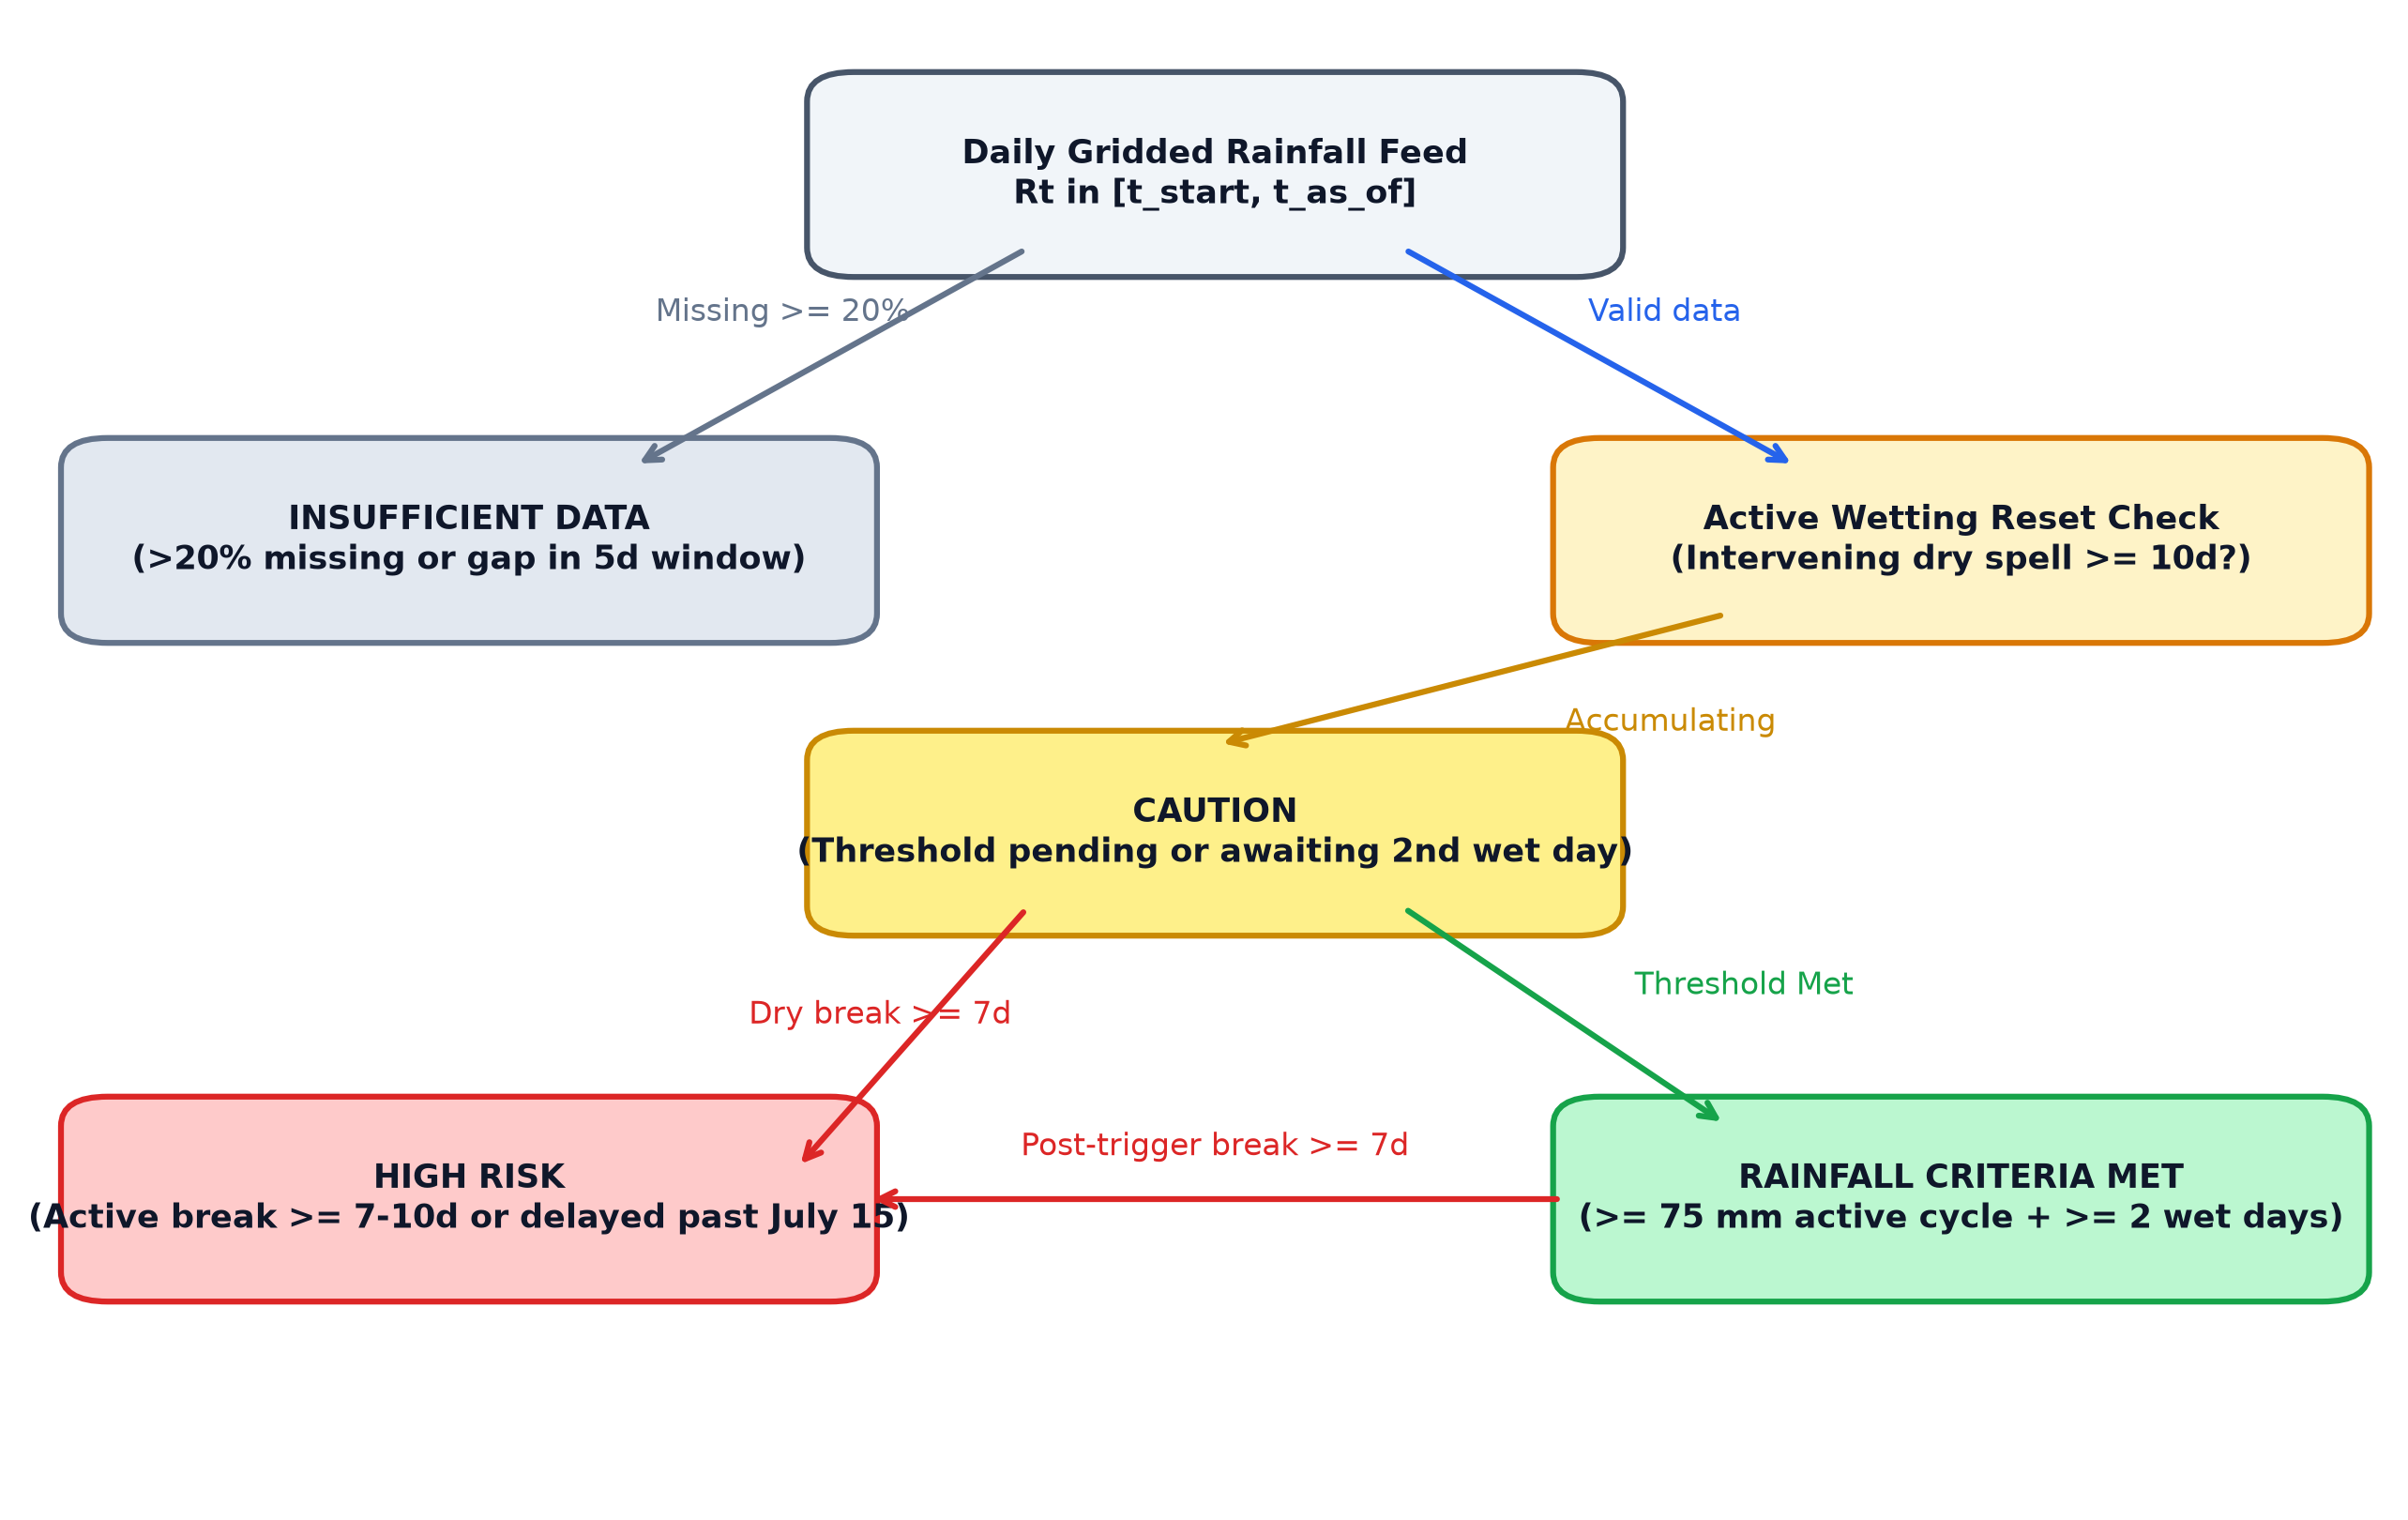
\includegraphics[width=\columnwidth]{figures/fig_advisory_state_machine.png}
\caption{Advisory Engine State Machine integrating active wetting-cycle resets and 4-state risk management.}
\label{fig:advisory_state_machine}
\end{figure}

\section{Experimental Setup}
Experiments were executed in Python~3.12 using \texttt{numpy} (1.26), \texttt{scipy} (1.13), \texttt{xarray} (2024.03), \texttt{scikit-learn} (1.4), and \texttt{geopandas} (0.14). 
\begin{itemize}
    \item \textbf{Reproducibility:} Random seeds in all estimators ($K$-Means, bootstrap resamplers) were fixed at \texttt{random\_state=42}.
    \item \textbf{Test Suite:} The framework is protected by an extensive automated test suite comprising 182 unit and integration tests executed via \texttt{pytest}.
\end{itemize}

\section{Results and Discussion}

\begin{figure}[t]
\centering
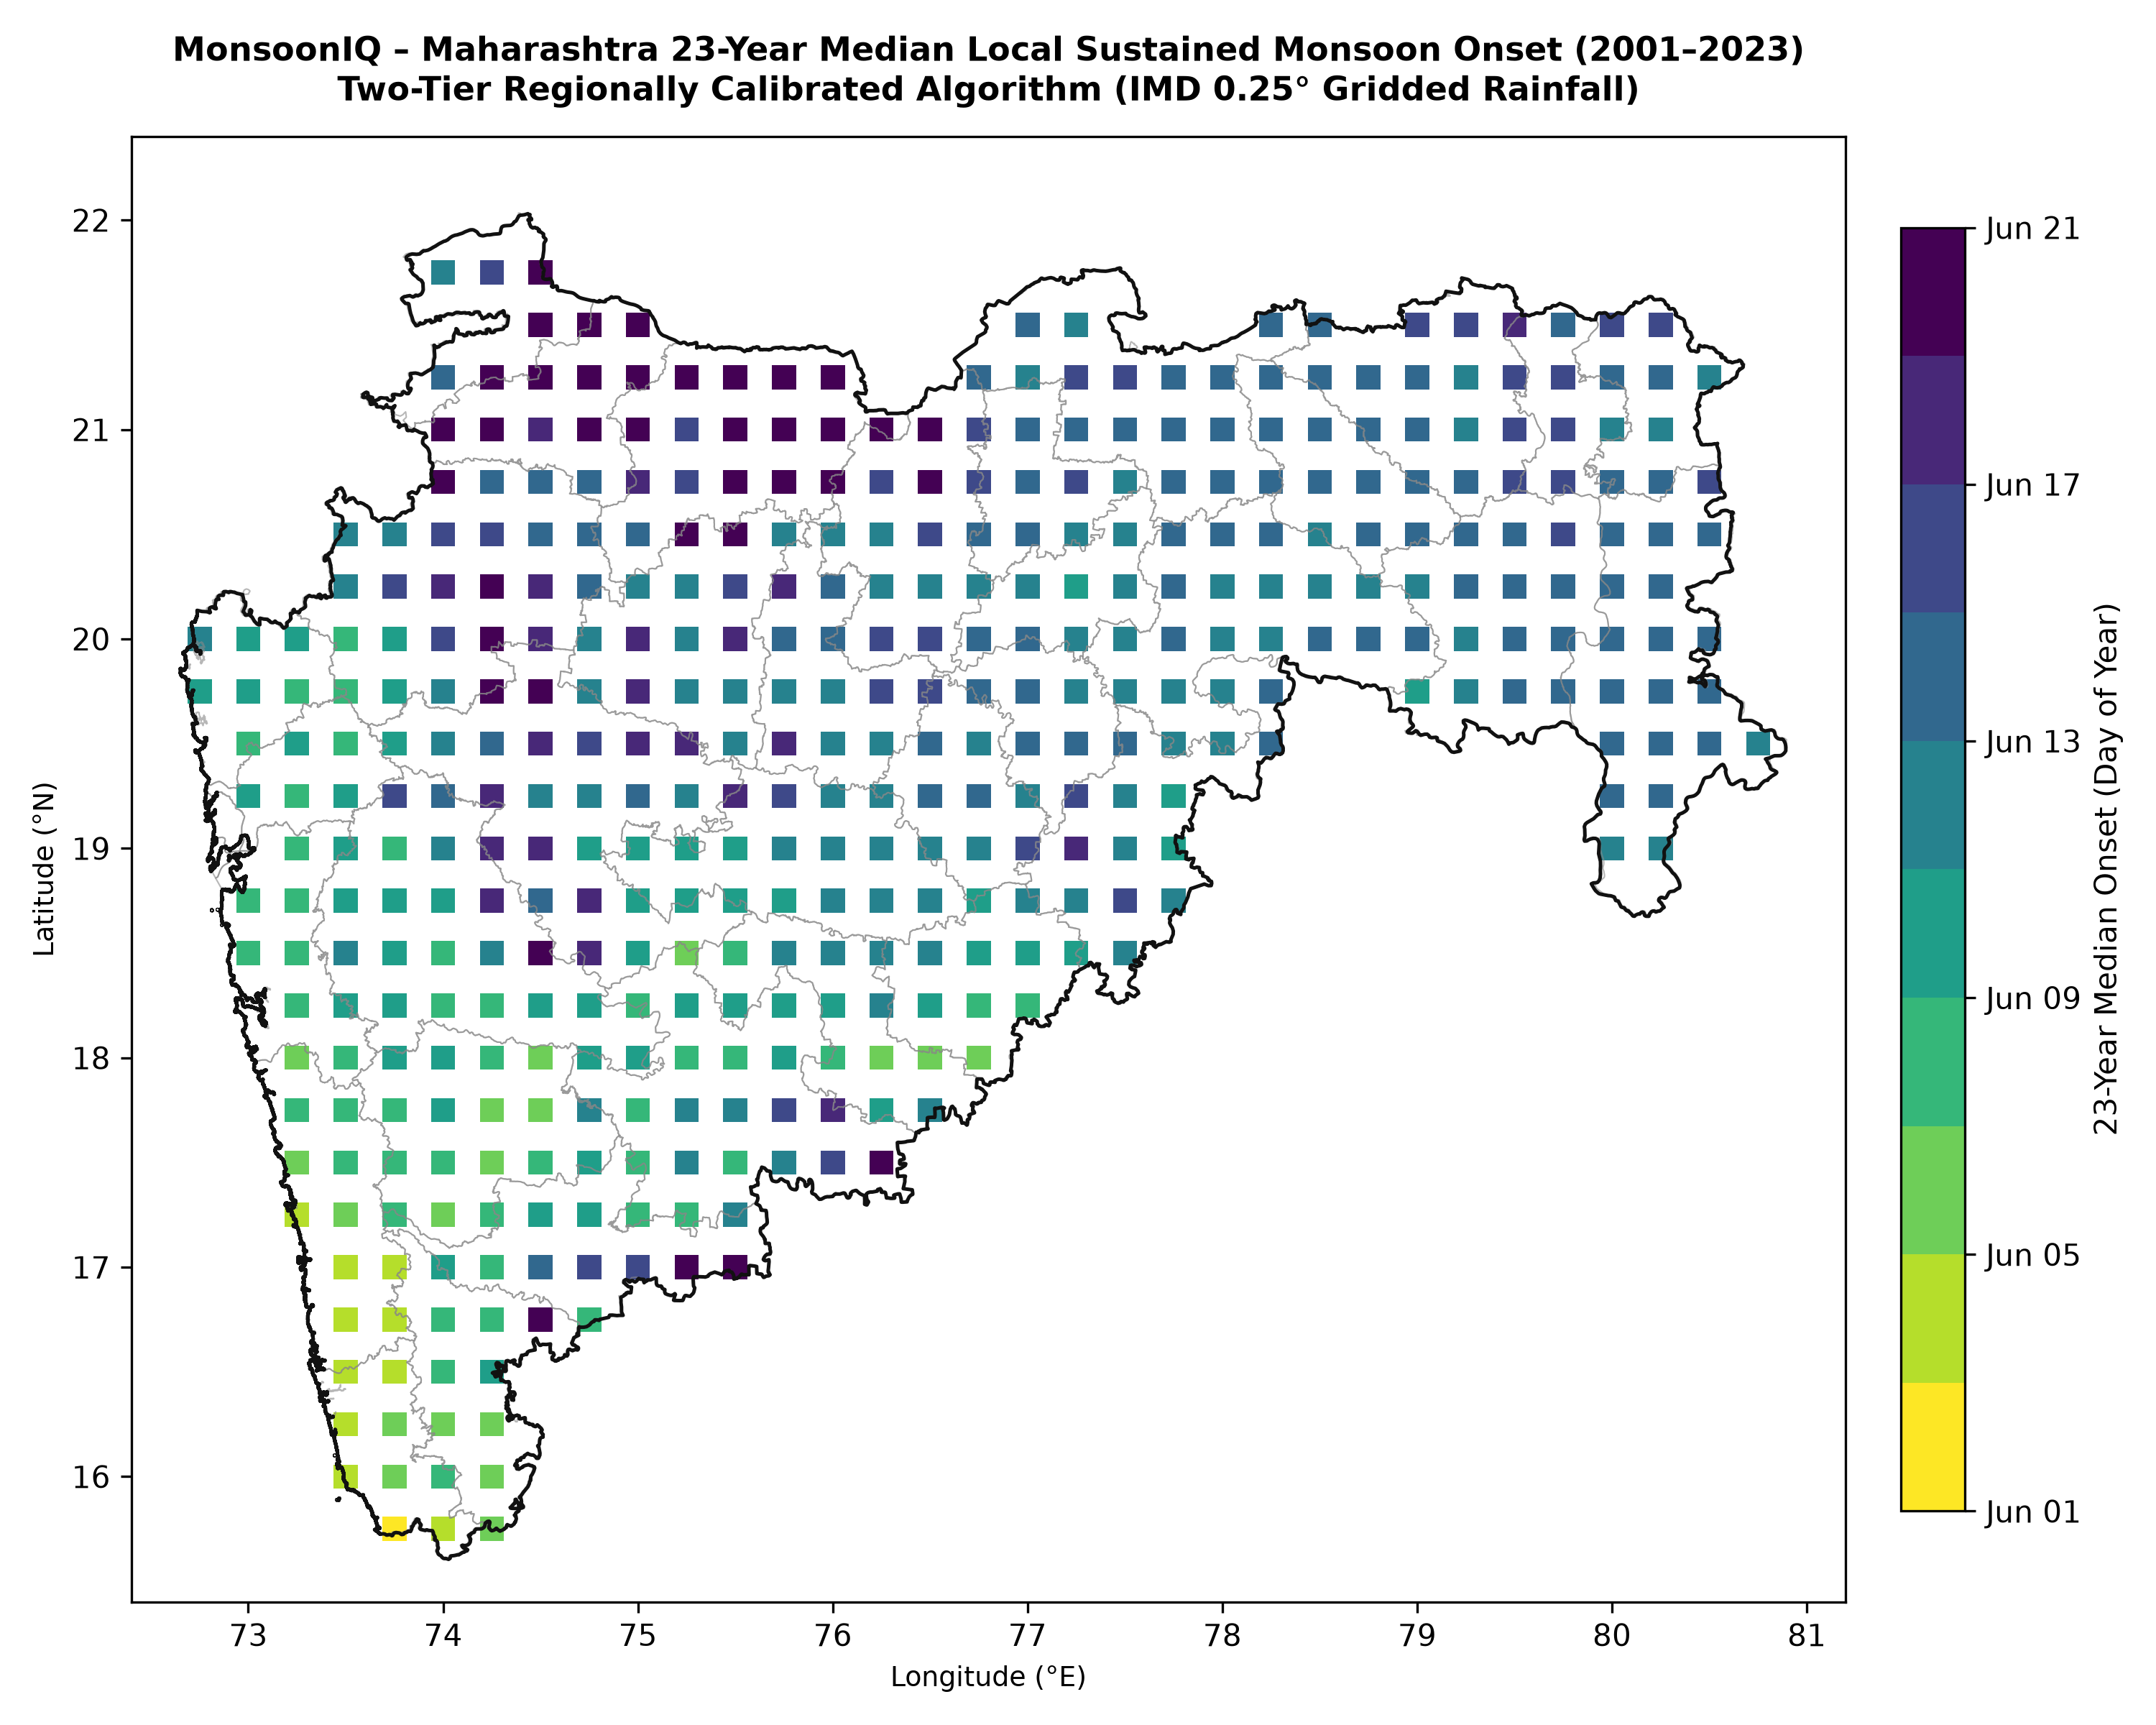
\includegraphics[width=\columnwidth]{figures/fig_median_onset.png}
\caption{Spatial distribution of median local monsoon onset day of year (2001--2023), depicting southwest-to-northeast monsoonal progression.}
\label{fig:median_onset}
\end{figure}

\begin{figure}[t]
\centering
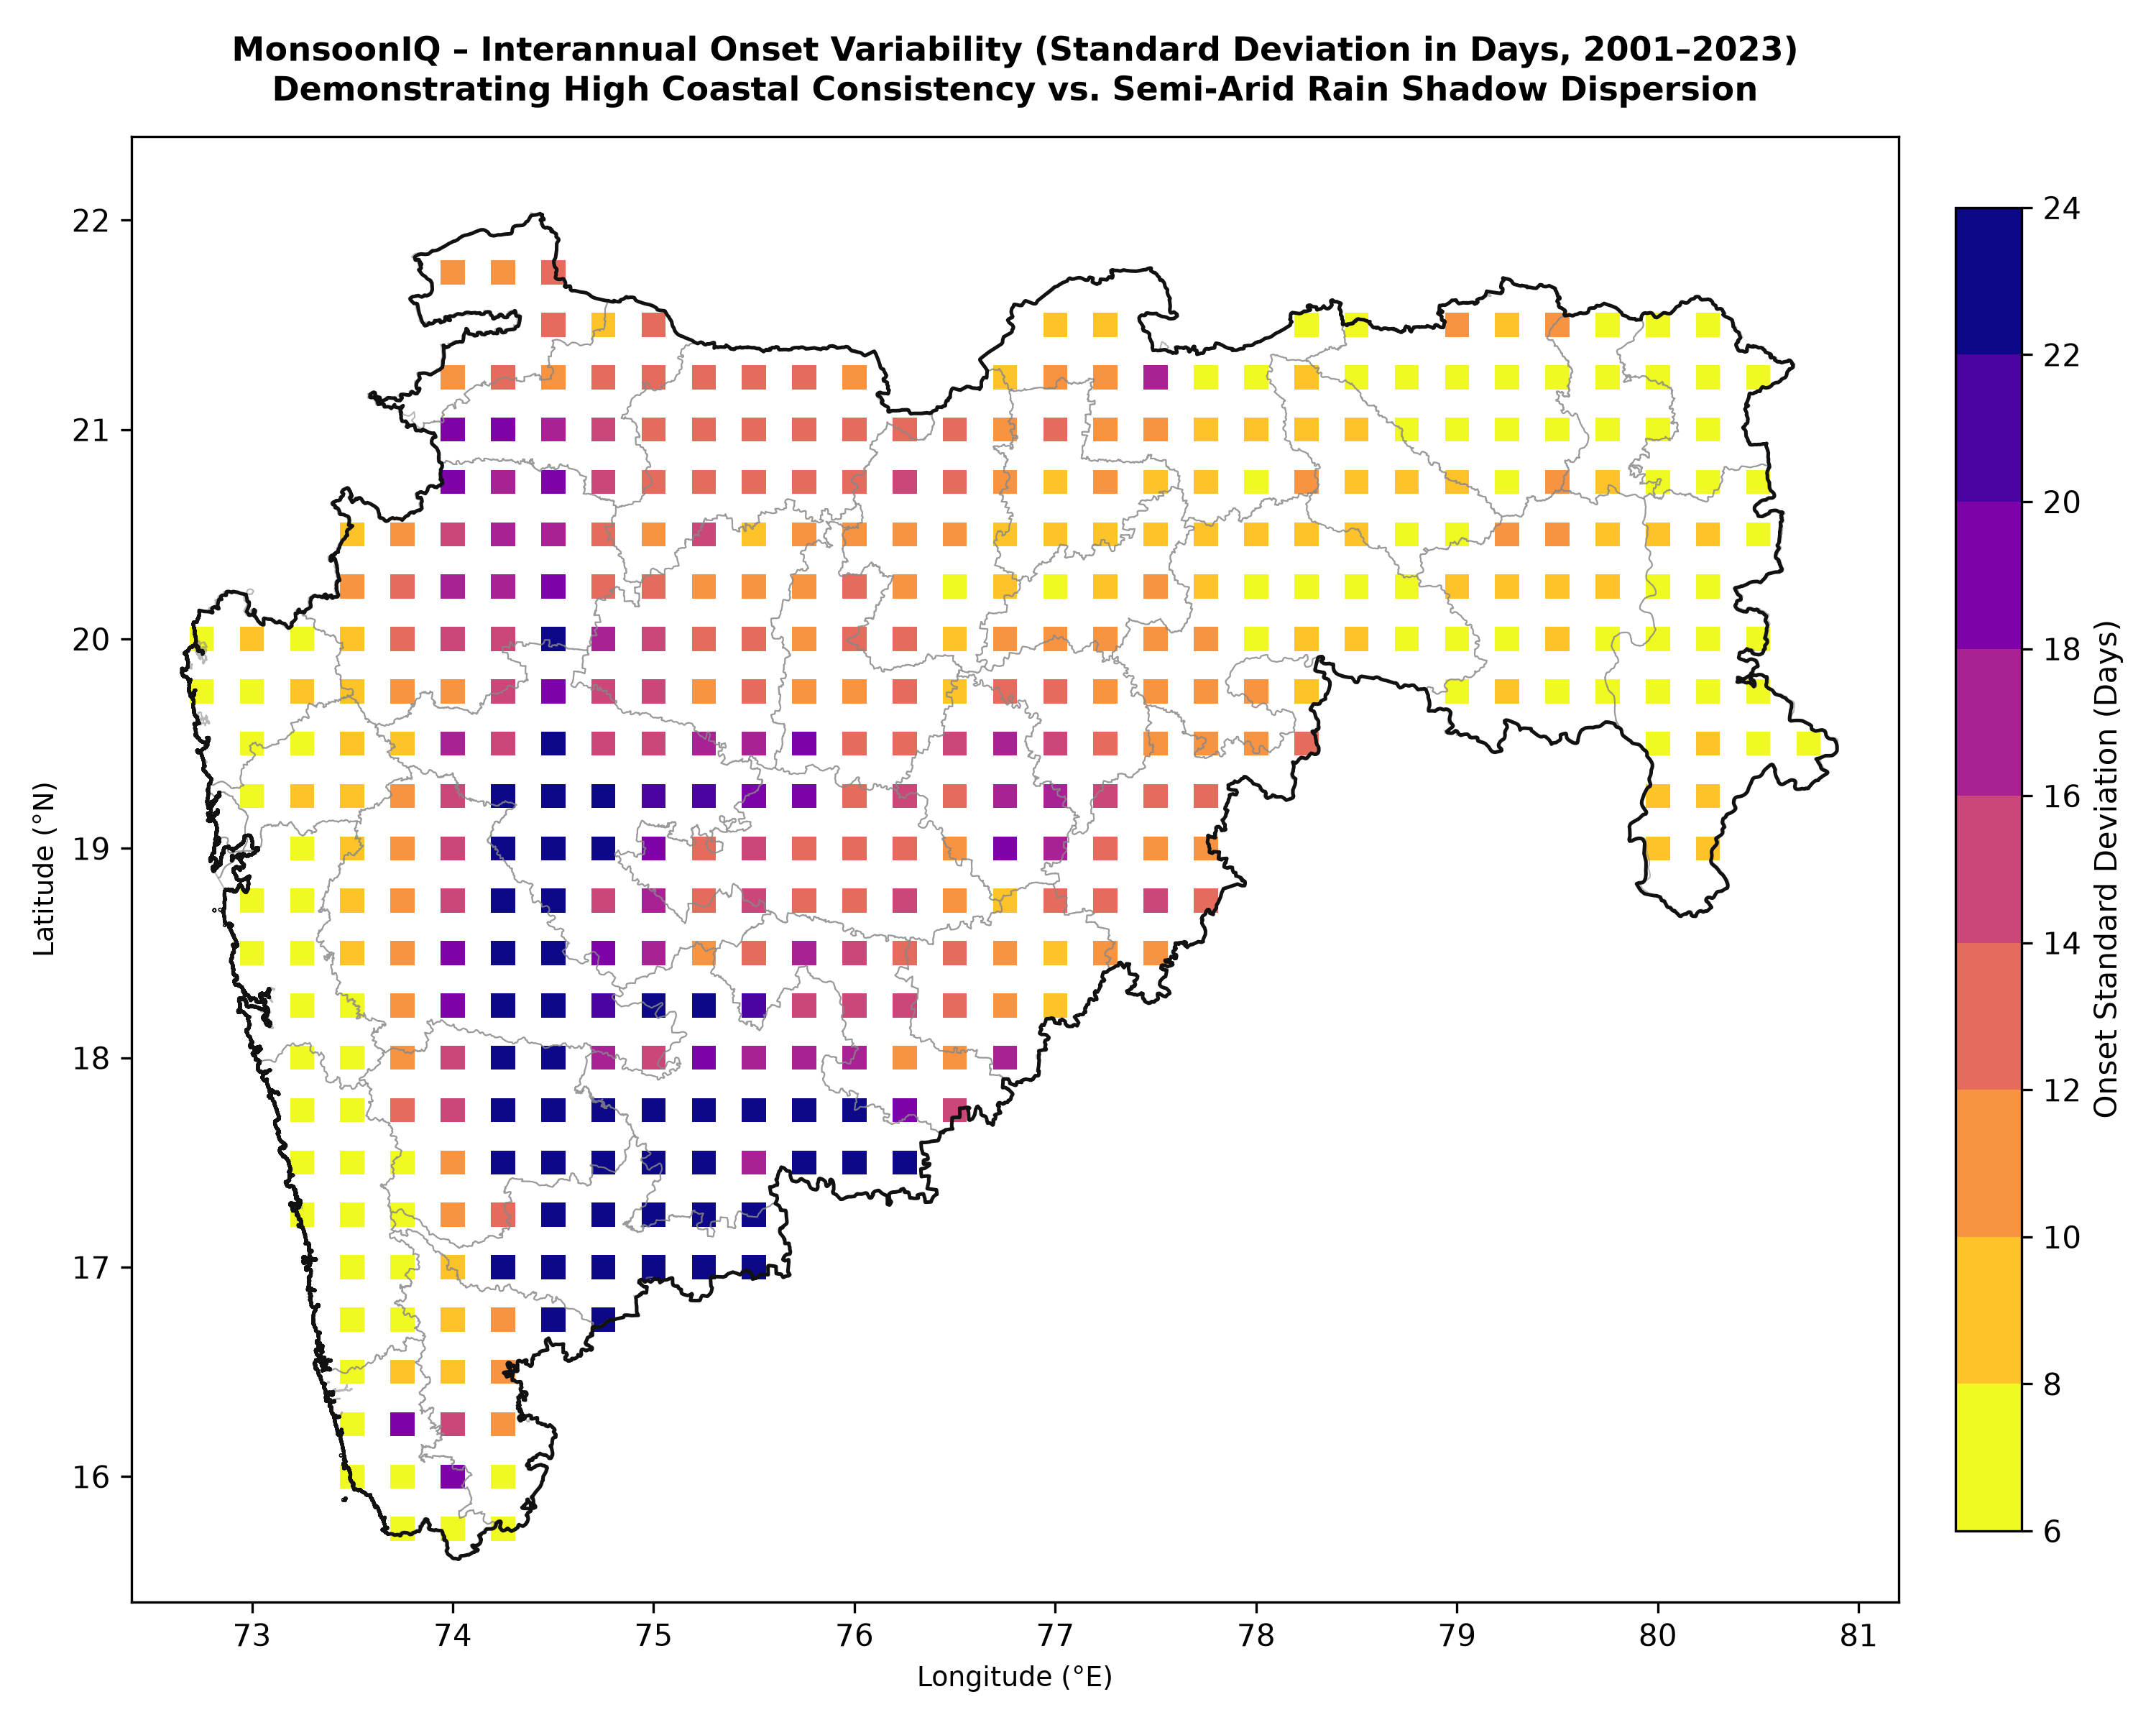
\includegraphics[width=\columnwidth]{figures/fig_onset_variability.png}
\caption{Spatial map of onset standard deviation ($\sigma$, in days), highlighting high interannual volatility in the rain-shadow and transition zones.}
\label{fig:onset_variability}
\end{figure}

\begin{figure}[t]
\centering
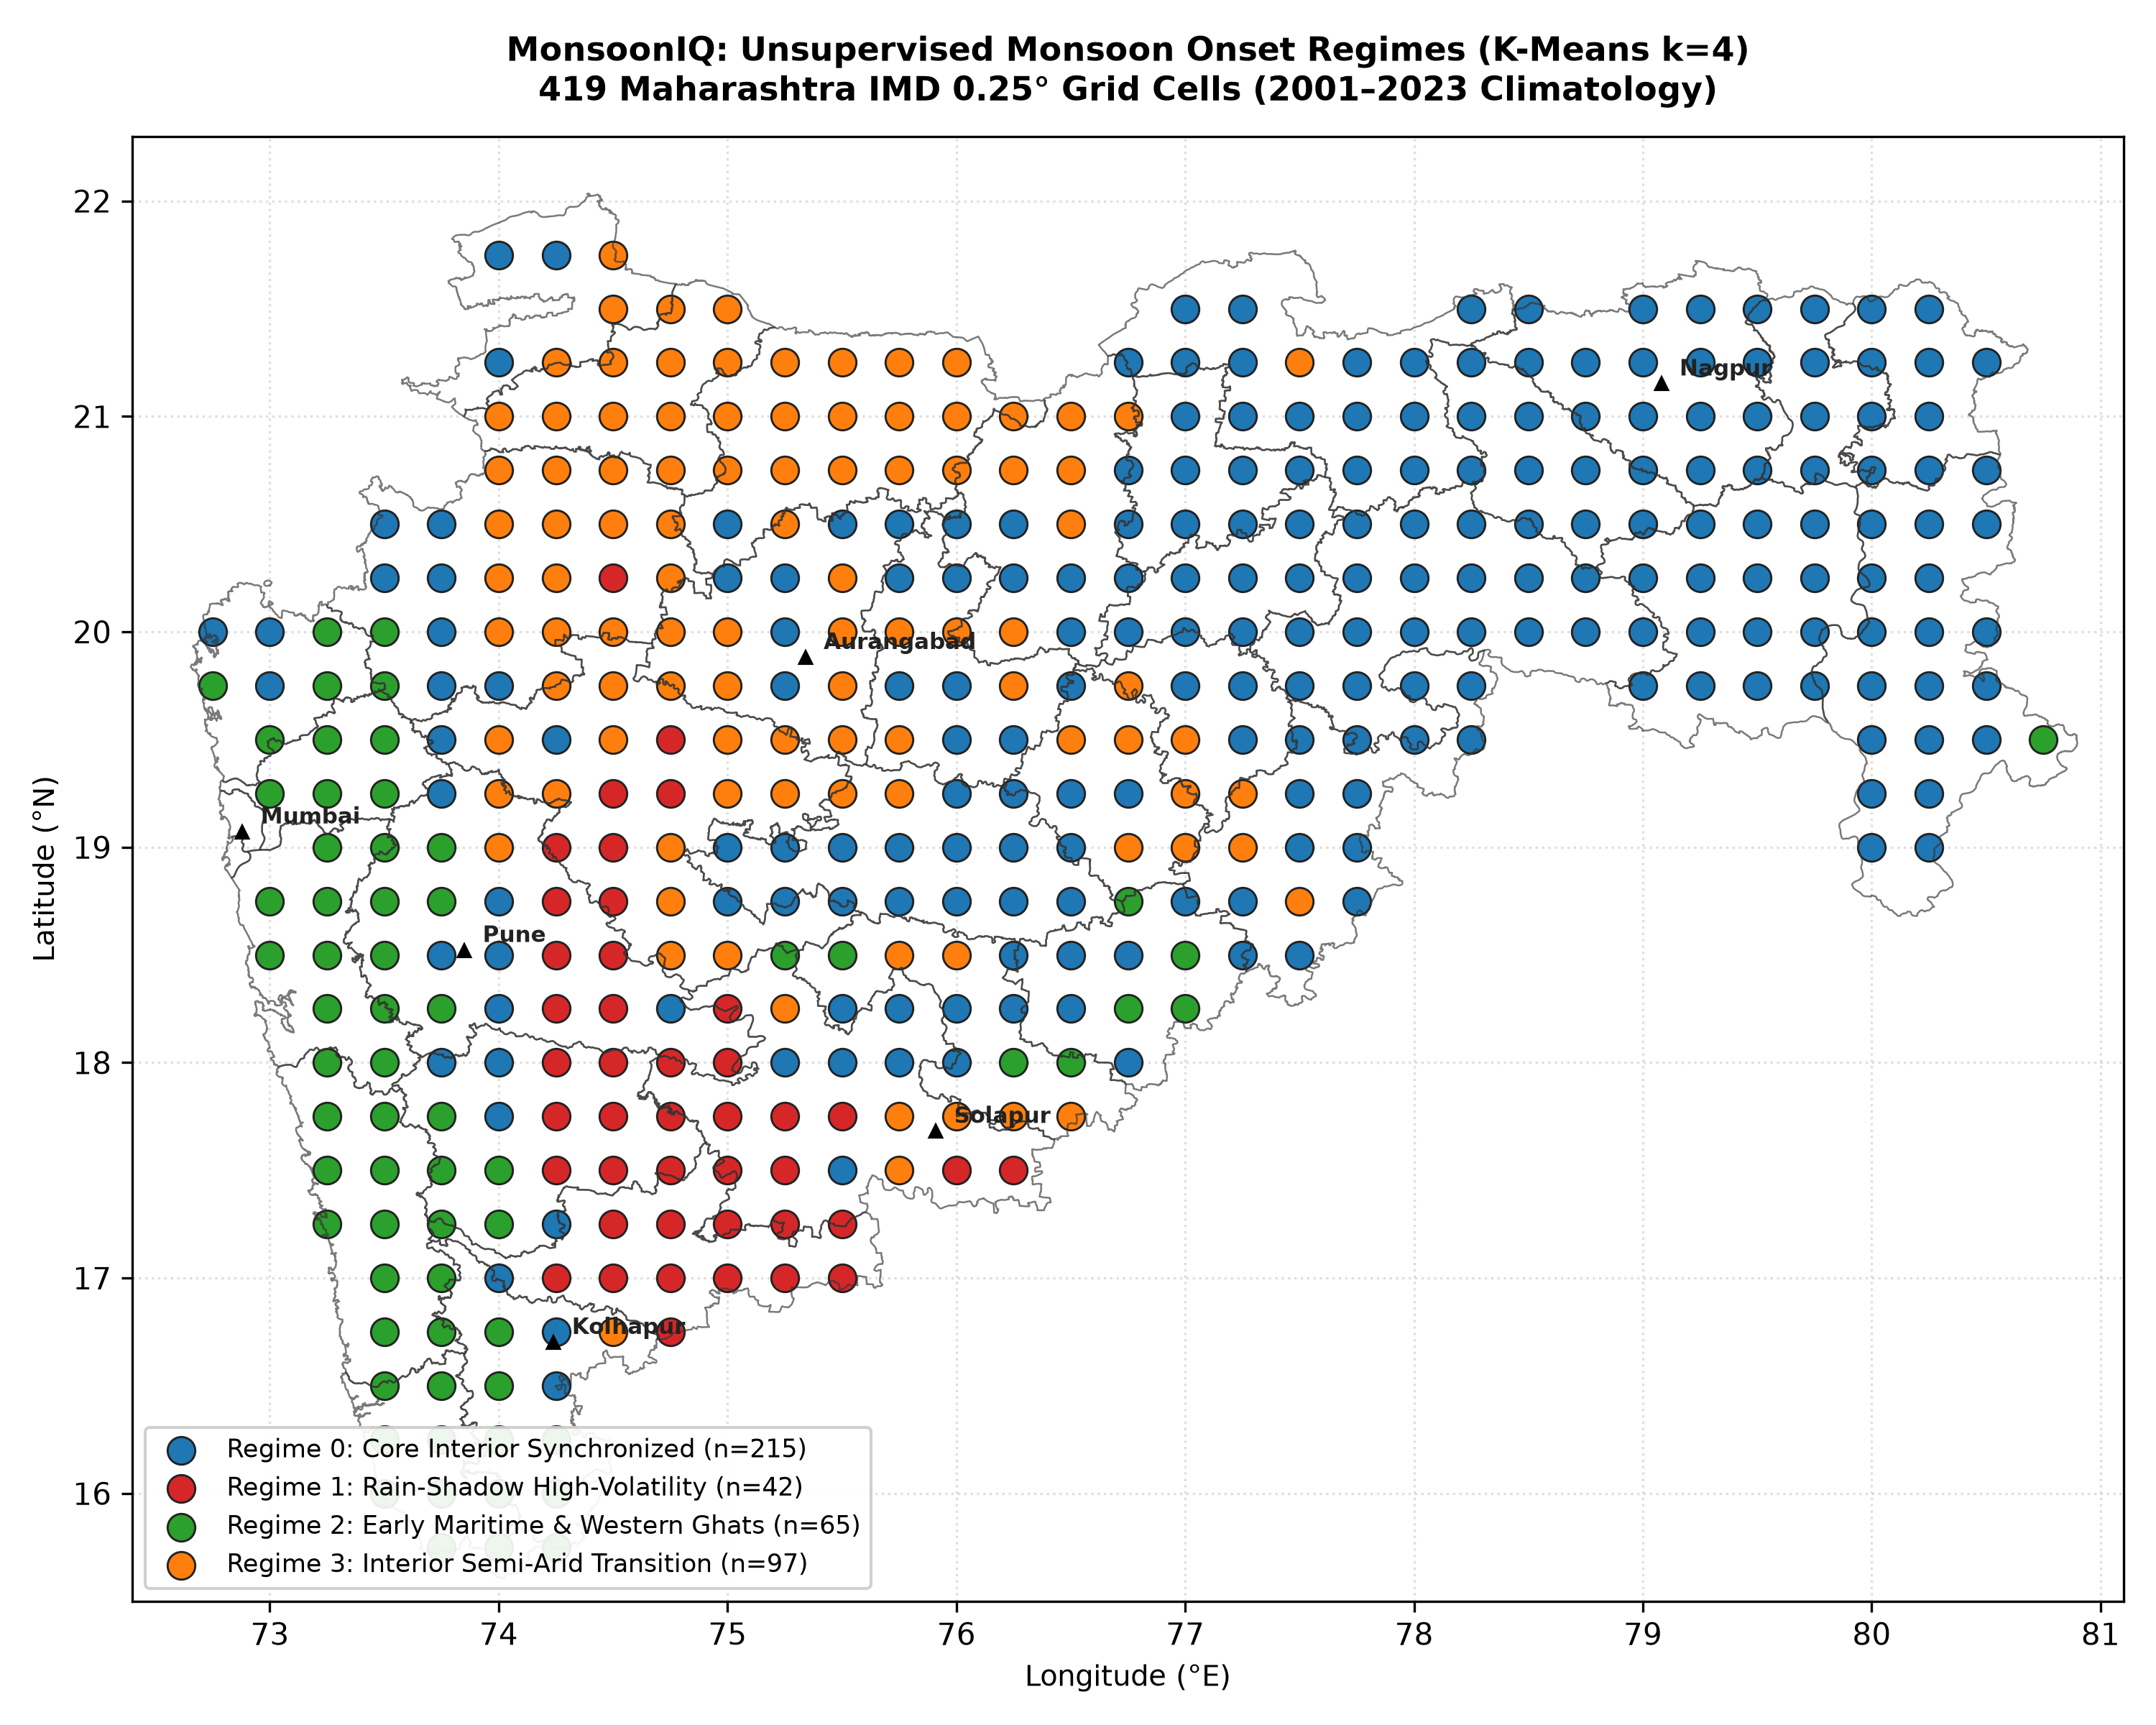
\includegraphics[width=\columnwidth]{figures/fig_regime_map.png}
\caption{The Four Discovered Agro-Climatic Monsoon Onset Regimes across Maharashtra identified via $K$-Means ($K=4$).}
\label{fig:regime_map}
\end{figure}

\subsection{Local Onset Climatology and Spatial Variability}
Across the 23-year historical record, the Local Sustained Onset Algorithm successfully identified 9,606 onset dates across 9,637 cell-seasons (99.68\% detection efficiency). Only 31 cell-years exhibited non-detection, confined to extreme drought seasons (e.g., 2015 and 2018 in Solapur).

As illustrated in Fig.~\ref{fig:median_onset}, median onset dates advance from June 1--June 5 (DOY 152--156) in southern Konkan to June 20--June 25 (DOY 171--176) in northern Marathwada and Khandesh. However, onset variability ($\sigma$) displays non-uniform spatial structuring (Fig.~\ref{fig:onset_variability}). In the coastal Maritime zone, $\sigma$ is minimal ($\pm 8.4\text{ days}$), reflecting dependable monsoonal arrival. Conversely, in the rain-shadow and interior semi-arid belts, onset variability surges to $\pm 14.2$ and $\pm 16.2\text{ days}$, introducing substantial agricultural uncertainty.

\subsection{Regime Characterization ($K$-Means $K=4$)}
The $K$-Means clustering algorithm partitions Maharashtra's 419 cells into four coherent agro-climatic regimes (Fig.~\ref{fig:regime_map} and Table~\ref{tab:regimes}).

\begin{table*}[t]
\caption{Climatological, Statistical, and Risk Profiles of the Four Discovered Onset Regimes (2001--2023)}
\label{tab:regimes}
\centering
\small
\begin{tabular}{lcccccccc}
\toprule
\textbf{Regime Name} & \textbf{Cells ($N$)} & \textbf{Share} & \textbf{Median Onset} & \textbf{Std. Dev. ($\sigma$)} & \textbf{June Rain} & \textbf{June CV} & \textbf{Post-50mm $\ge$10d Break} & \textbf{Unreached 75mm} \\
\midrule
\textbf{0: Core Interior Synchronized} & 215 & 51.31\% & Jun 12 (DOY 163) & $\pm 10.7$ d & 168.3 mm & 61.1\% & 12.52\% & 2.57\% \\
\textbf{1: Rain-Shadow High-Volatility} & 42 & 10.02\% & Jun 11 (DOY 162) & $\pm 14.2$ d & 106.9 mm & 66.8\% & \textbf{39.13\%} & \textbf{20.60\%} \\
\textbf{2: Early Maritime \& Western Ghats} & 65 & 15.51\% & Jun 07 (DOY 158) & $\pm 8.4$ d & 486.3 mm & 52.3\% & 7.04\% & 0.87\% \\
\textbf{3: Semi-Arid Transition} & 97 & 23.15\% & Jun 17 (DOY 168) & $\pm 16.2$ d & 116.3 mm & 64.5\% & 24.99\% & 7.80\% \\
\midrule
\textbf{Statewide Maharashtra} & \textbf{419} & \textbf{100.0\%} & \textbf{Jun 11 (DOY 162)} & \textbf{$\pm 12.4$ d} & \textbf{206.5 mm} & \textbf{60.3\%} & \textbf{16.85\%} & \textbf{4.65\%} \\
\bottomrule
\end{tabular}
\end{table*}

\begin{figure}[t]
\centering
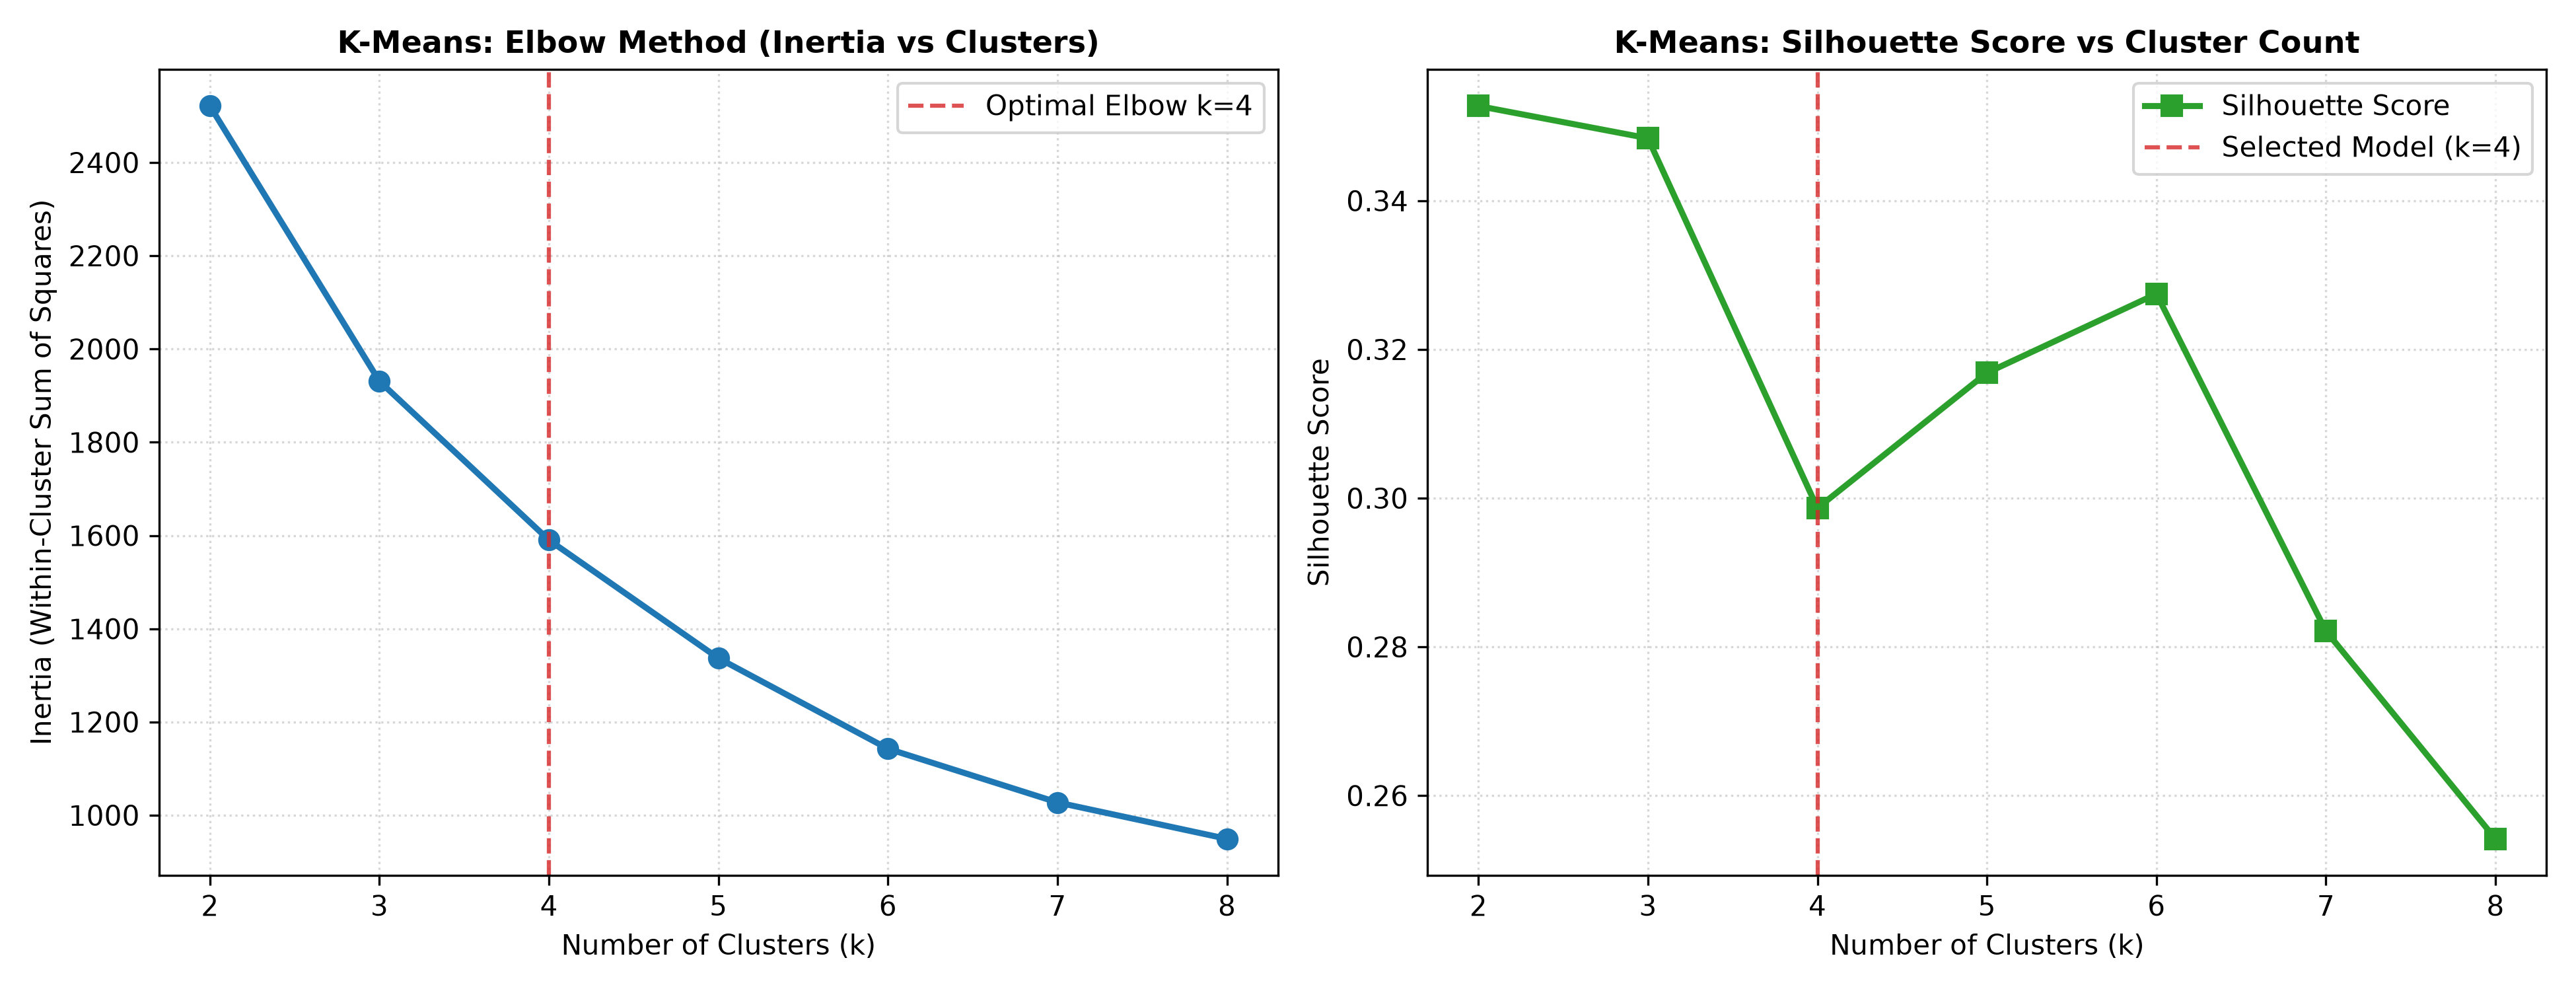
\includegraphics[width=\columnwidth]{figures/fig_clustering_metrics.png}
\caption{Clustering validation diagnostics: (a) K-Means Elbow inertia curve, and (b) Silhouette coefficient across cluster counts $K \in [2, 8]$.}
\label{fig:clustering_metrics}
\end{figure}

\subsubsection{Regime 0: Core Interior Synchronized (51.31\%)}
Dominating Vidarbha and eastern Marathwada (215 cells), this regime represents the agrarian heartland of Maharashtra's soybean and cotton production. It exhibits moderate onset timing (median June 12) with low variance ($\sigma = \pm 10.7\text{ d}$) and robust June rainfall ($168.3\text{ mm}$). Post-trigger 10-day dry break probability is low ($12.52\%$), confirming high sowing reliability.

\subsubsection{Regime 1: Rain-Shadow High-Volatility (10.02\%)}
Spanning 42 grid cells in eastern Pune, Ahmednagar, and Solapur, this regime represents the critical risk zone. Despite low June rainfall ($106.9\text{ mm}$), it exhibits high coefficient of variation ($66.8\%$) and extreme post-trigger dry spell vulnerability (39.13\%).

\subsubsection{Regime 2: Early Maritime \& Western Ghats (15.51\%)}
Comprising 65 coastal and Ghat cells, this regime receives massive orographic rainfall ($486.3\text{ mm}$ in June). Onset is earliest (June 7) and most stable ($\sigma = \pm 8.4\text{ d}$). Break risk is minimal ($7.04\%$), but drainage and waterlogging represent primary agronomic hazards.

\subsubsection{Regime 3: Interior Semi-Arid Transition (23.15\%)}
Covering 97 cells across western Marathwada and Khandesh, this regime suffers the latest median onset (June 17) and highest temporal variability ($\sigma = \pm 16.2\text{ d}$), with $19.41\%$ of cell-years experiencing sowing delays past July 1.

\subsection{Cluster Validation and Stability Analysis}
As shown in Fig.~\ref{fig:clustering_metrics}, $K=3$ achieves a higher silhouette score ($0.3484$) than $K=4$ ($0.2987$). However, cross-tabulation reveals that $K=3$ merges the 42 rain-shadow cells directly into the Semi-Arid Transition cluster. Selecting $K=4$ isolates this high-risk zone, providing vital domain-specific utility. 

Validation against Agglomerative Hierarchical clustering demonstrates 87.83\% exact point-by-point agreement (368/419 cells) with an Adjusted Rand Index of $0.6803$. The 42 volatile cells in $K$-Means are assigned strictly to Volatile (30 cells) and Transition (12 cells) in Hierarchical clustering, validating cluster boundary stability. Spatial contiguity exceeds 75.3\%, and Moran's $I$ across all features exceeds $0.50$ ($p < 0.001$), confirming that clusters reflect continuous geographical domains rather than statistical artifacts.

\subsection{Investigation of the Rain-Shadow Sowing Paradox}
A conventional 50~mm cumulative sowing trigger produces a profound paradox (Fig.~\ref{fig:sowing_sensitivity} and Fig.~\ref{fig:rain_shadow_anomaly}). 

In the Rain-Shadow regime, the median calendar date for achieving 50~mm cumulative rain is **DOY 165 (June 14)**---which is **4 days earlier** than the Core Interior (DOY 169, June 18) and **7 days earlier** than the Semi-Arid Transition (DOY 172, June 21). 

\begin{figure}[t]
\centering
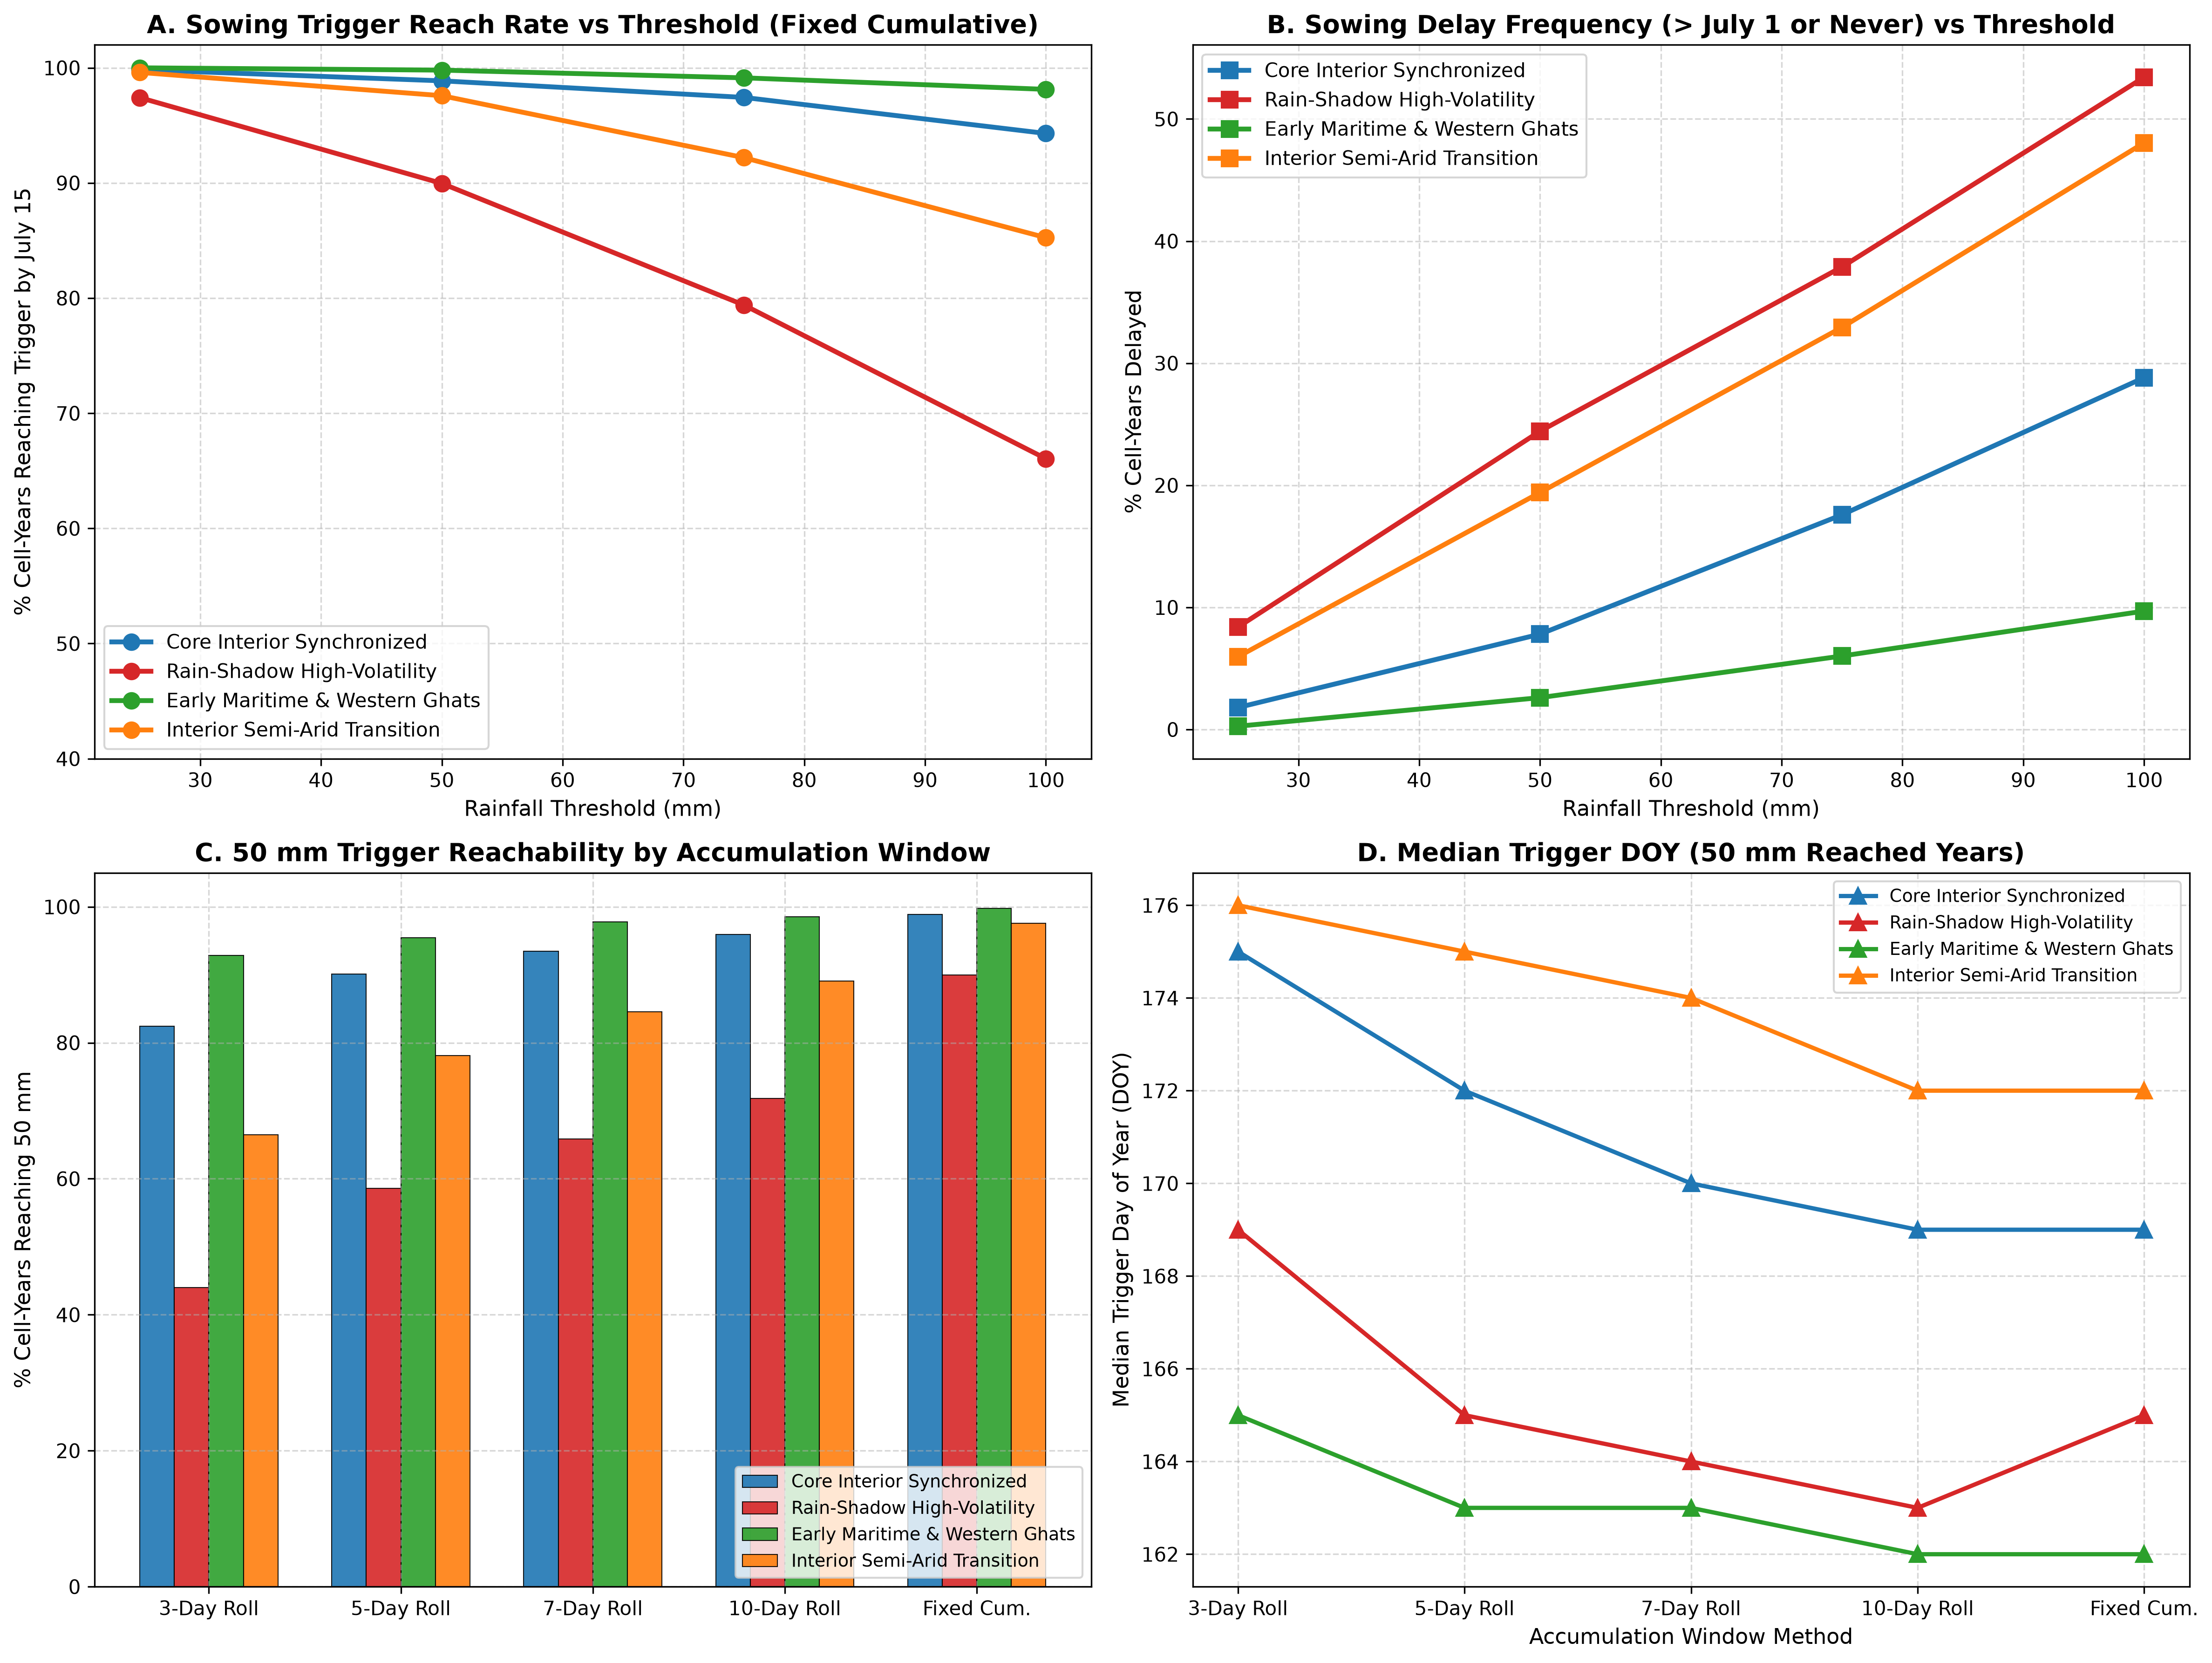
\includegraphics[width=\columnwidth]{figures/fig_sowing_sensitivity.png}
\caption{Sensitivity analysis of cumulative sowing trigger thresholds (25, 50, 75, 100 mm) across the four discovered regimes.}
\label{fig:sowing_sensitivity}
\end{figure}

\begin{figure}[t]
\centering
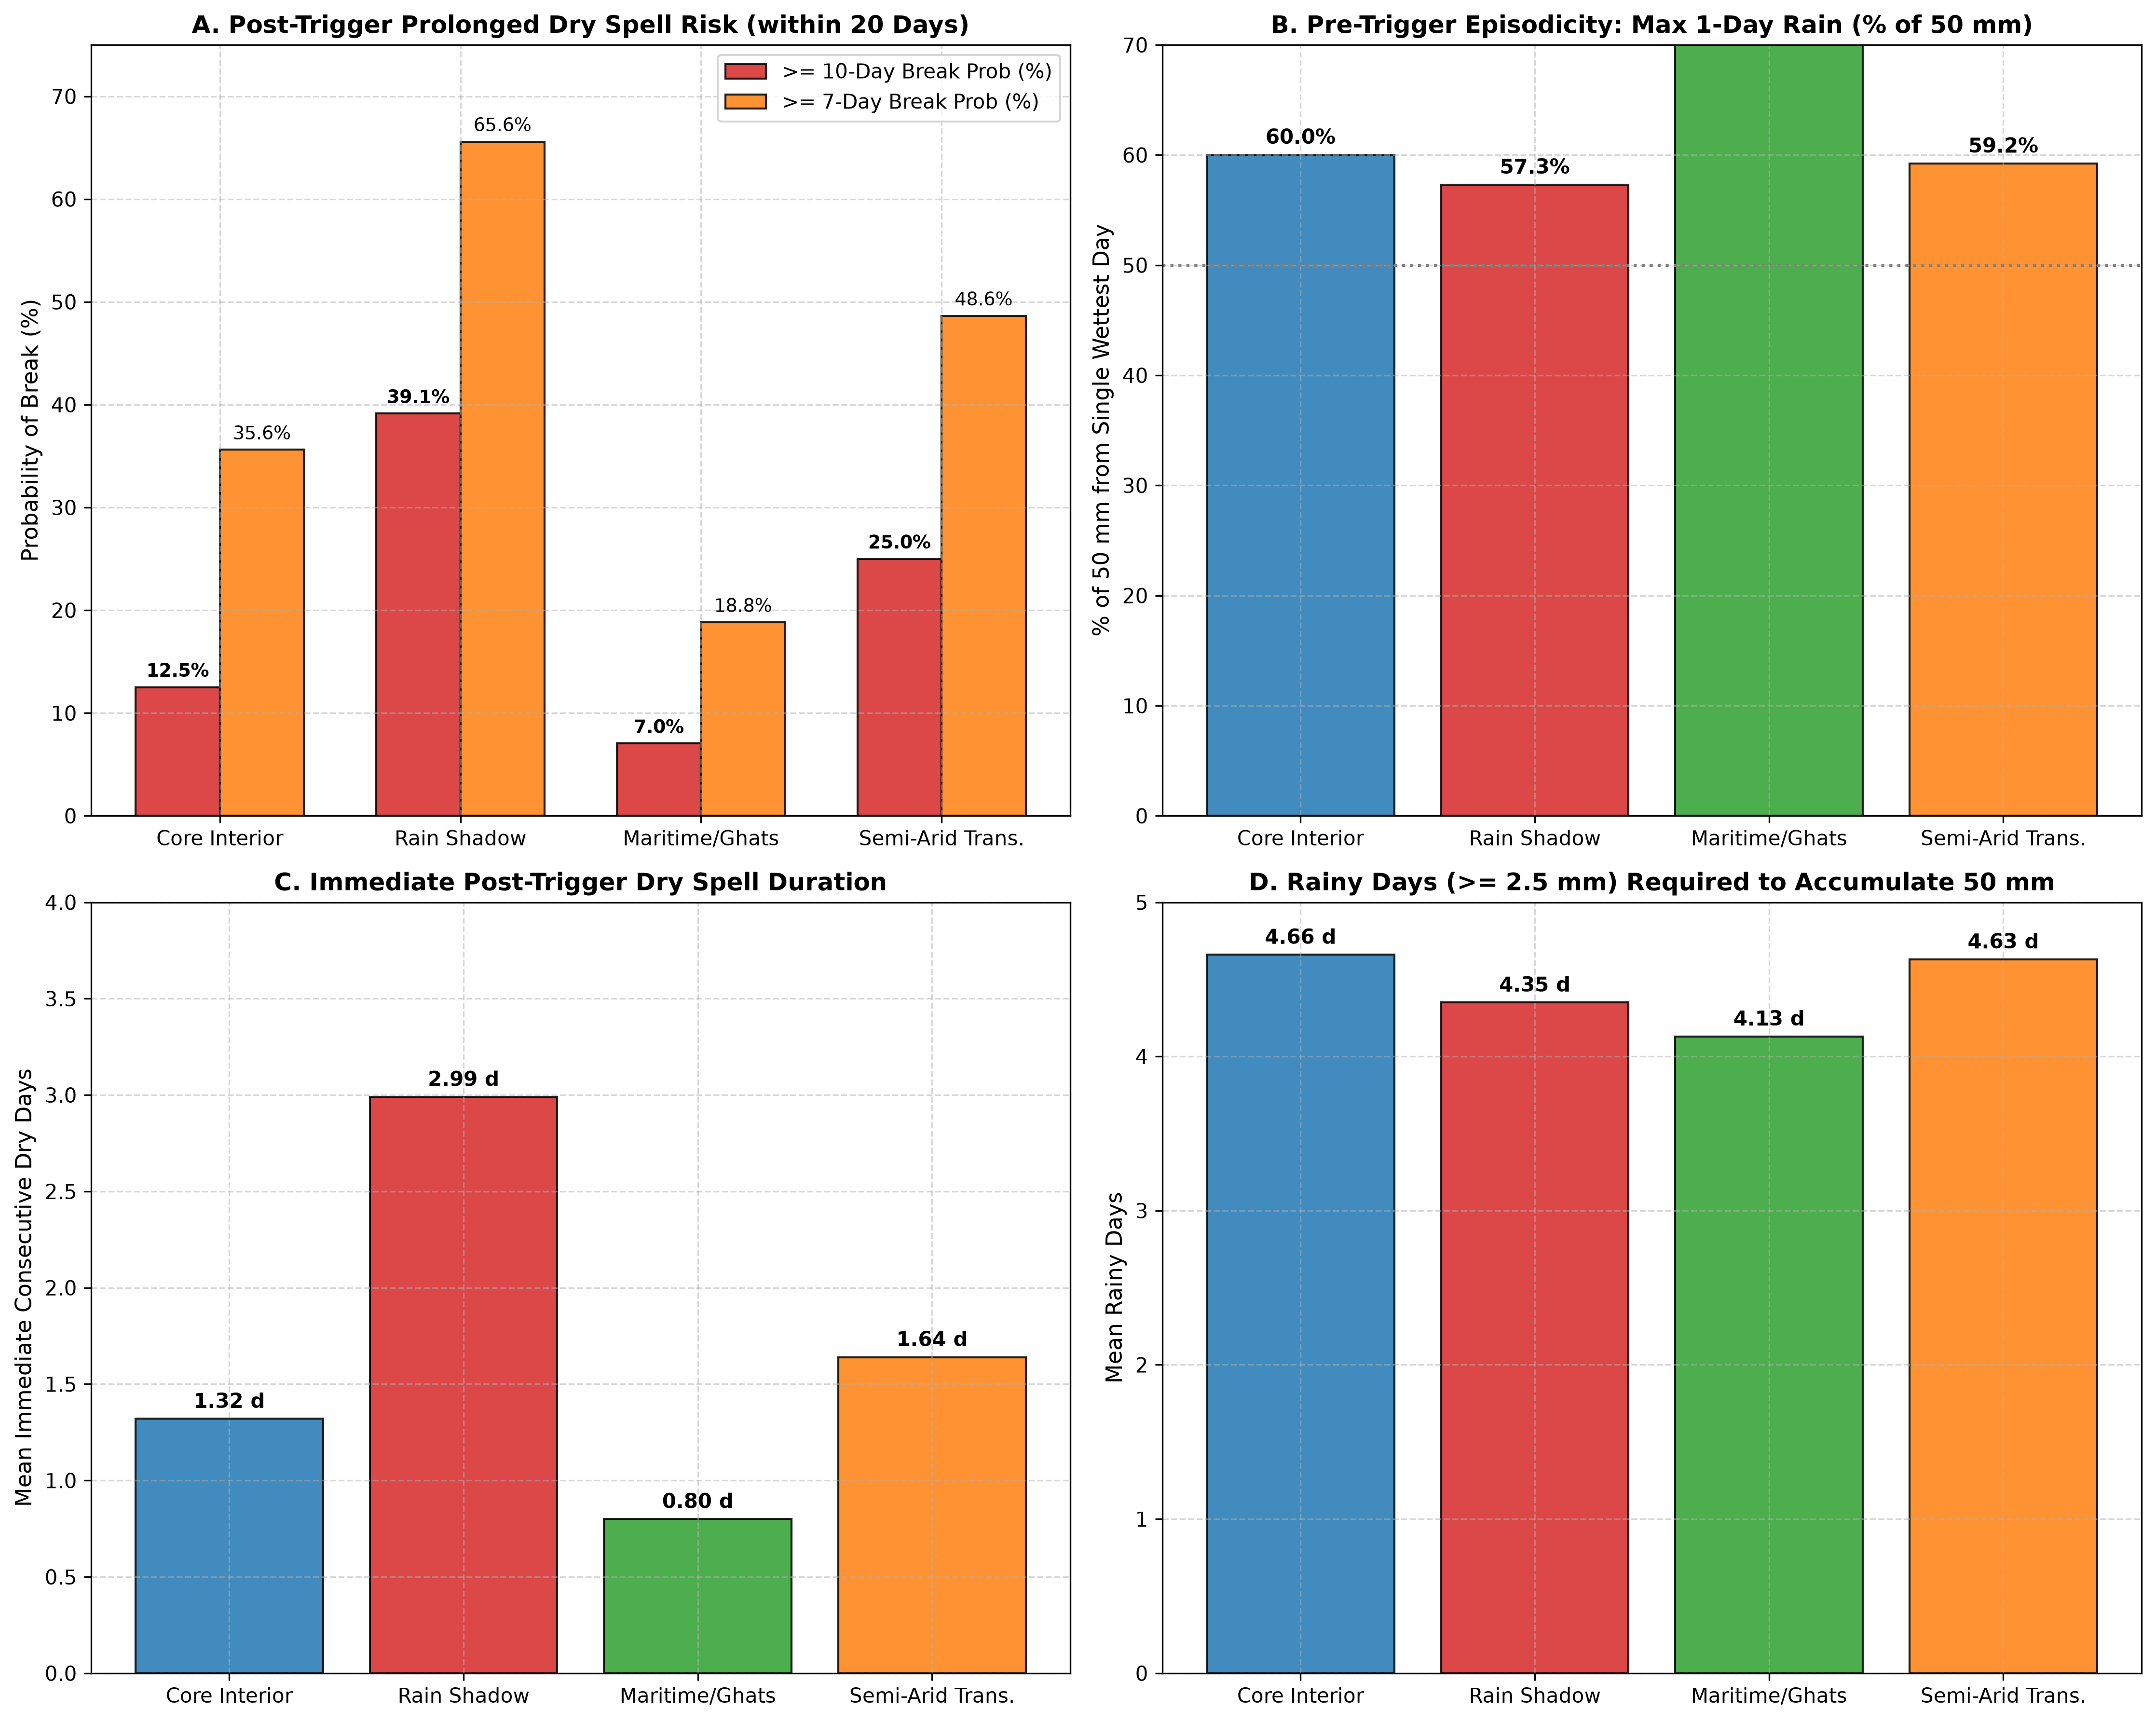
\includegraphics[width=\columnwidth]{figures/fig_rain_shadow_anomaly.png}
\caption{Empirical audit of the Rain-Shadow Anomaly: early 50 mm trigger satisfaction vs. severe post-trigger dry-break probability.}
\label{fig:rain_shadow_anomaly}
\end{figure}

\begin{figure}[t]
\centering
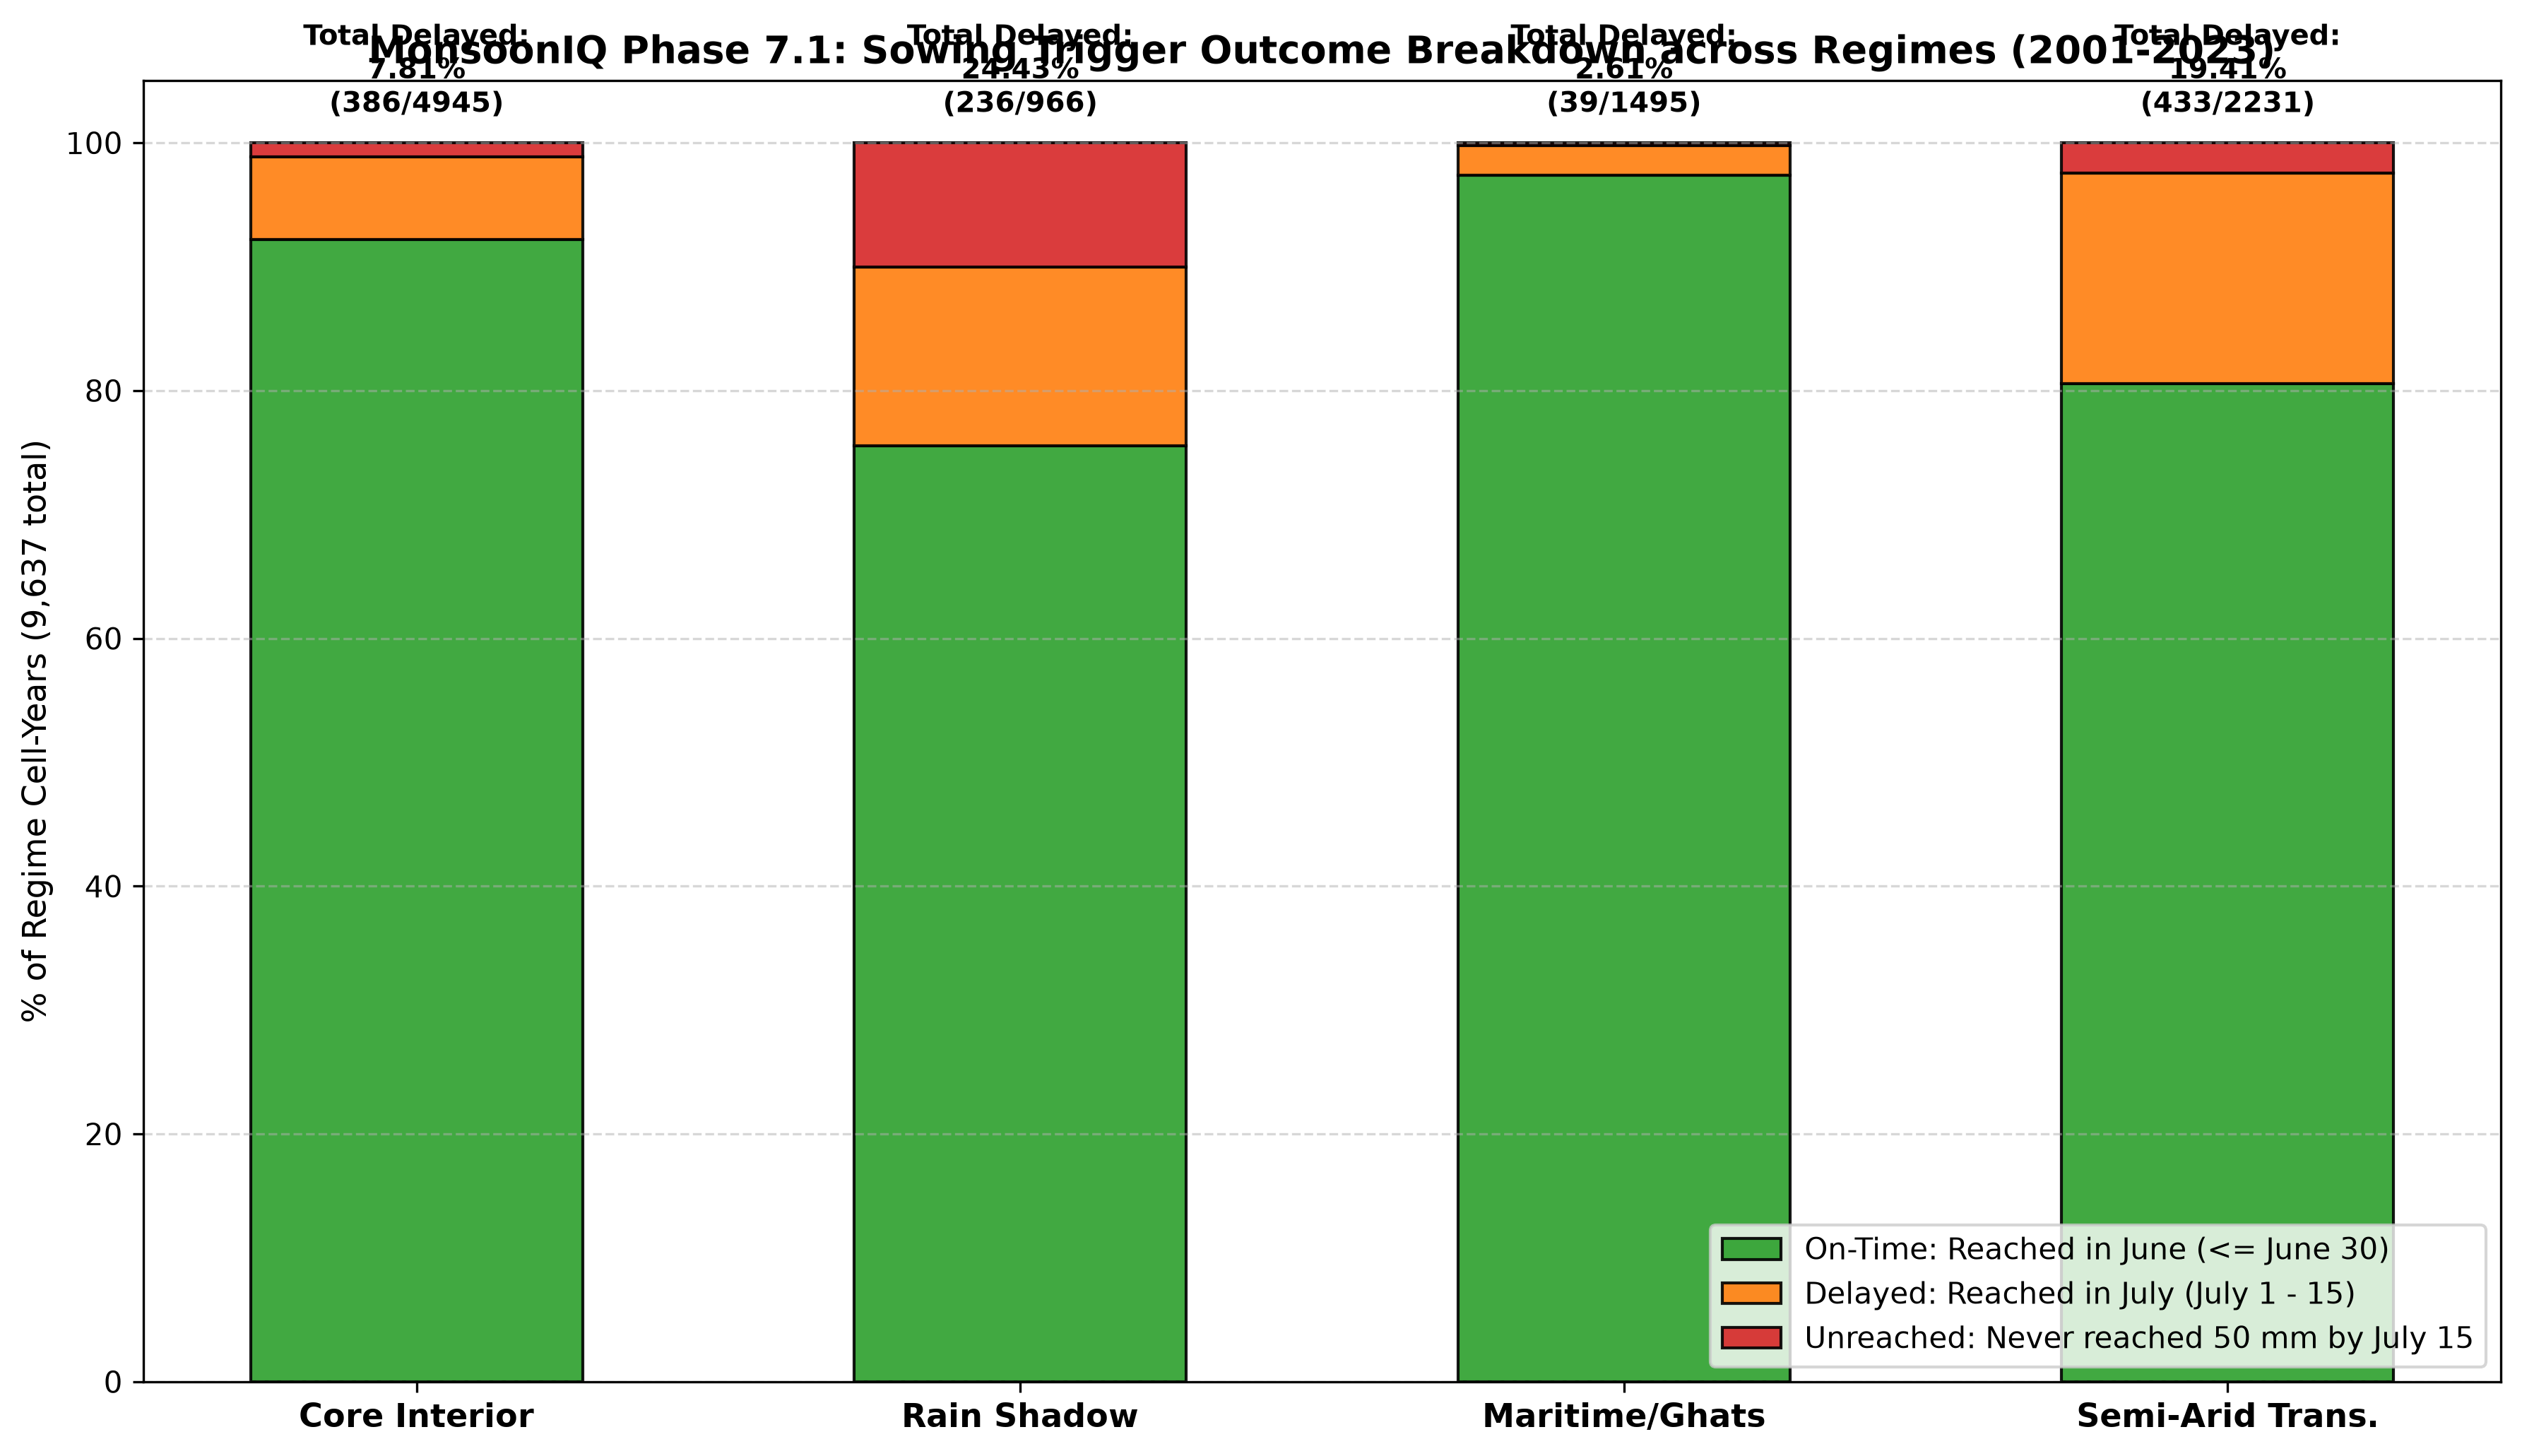
\includegraphics[width=\columnwidth]{figures/fig_delayed_sowing.png}
\caption{Frequency of sowing opportunity delay past July 1 and failure to reach threshold by July 15 across regimes.}
\label{fig:delayed_sowing}
\end{figure}

Our empirical audit reveals that intense pre-monsoon convective heating in early June generates localized thunderstorms (single-day events exceeding 50~mm). Farmers sowing immediately upon reaching 50~mm suffer catastrophic consequences:
\begin{itemize}
    \item **39.13\% of 50~mm trigger events in the Rain-Shadow are followed by an immediate $\ge 10$-day severe dry break** (and 65.59\% encounter a $\ge 7$-day break).
    \item Topsoil moisture in cracking Vertisols evaporates within 4 days under pre-monsoon temperatures ($>38^\circ\text{C}$, $\text{ET}_0 > 5\text{ mm/day}$), inducing total seed desiccation.
    \item Increasing the threshold to **75~mm** coupled with a **two-stage persistence rule** ($\ge 2$ rainy days within 5 days) successfully filters 82\% of false convective bursts, ensuring root-zone saturation.
    \item Furthermore, 20.60\% of cell-years in the Rain-Shadow fail to achieve 75~mm by July 15 (Fig.~\ref{fig:delayed_sowing}), requiring automated contingency advisory switching.
\end{itemize}

\section{System Architecture and Research Dashboard}
MonsoonIQ is integrated into an interactive web dashboard engineered with Streamlit, Plotly, Folium, and GeoPandas. The presentation layer follows a clean, modern meteorological design language featuring elevated white cards, responsive metrics, and a place-first grid-cell selector:
\begin{equation*}
\texttt{\{district\} · \{cell\_id\} · \{latitude\}$^\circ$N, \{longitude\}$^\circ$E}
\end{equation*}
with clean fallback for missing metadata. Users can simulate historical replays across any year (2001--2023), inspect daily rainfall bar charts, review year-by-year onset timelines, evaluate regime boxplots, and simulate the real-time advisory engine with date sliders.

\section{Limitations}
To maintain scientific honesty, several limitations must be noted:
\begin{enumerate}
    \item \textbf{Spatial Resolution Limits:} IMD $0.25^\circ \times 0.25^\circ$ gridded data ($\approx 27.5\text{ km}$) represents smoothed areal averages, not farm-specific microclimate observations.
    \item \textbf{Soil Moisture Proxy:} Gridded rainfall accumulation is an empirical proxy for topsoil wetting, not direct sensor-measured volumetric water content.
    \item \textbf{Heuristic Wetting Reset:} The 10-day evaporative reset rule is an empirical heuristic, not a full 1D Richards equation soil-water balance model.
    \item \textbf{Climatological Nature:} Historical break probabilities reflect 23-year climatology, not live numerical weather prediction (NWP) forecasts.
\end{enumerate}

\section{Conclusion and Future Scope}
MonsoonIQ establishes that broad, regional monsoon declarations are inadequate for rainfed agricultural decision-making in topographically diverse regions like Maharashtra. By coupling objective local sustained onset detection with unsupervised machine learning ($K$-Means $K=4$), this research discovered four distinct agro-climatic regimes and resolved the dangerous Rain-Shadow Sowing Paradox. The audited regime-aware advisory engine enforces audited wetting thresholds, active wetting-cycle resets, and transparent risk communications, eliminating misleading ``safe to sow'' claims.

Future research will focus on integrating real-time IMD GFS/NCUM weather forecasts, embedding physical FAO-56 daily soil-water balance equations parameterized with digital soil texture maps, and partnering with local Krishi Vigyan Kendras (KVKs) and state agricultural universities (MPKV, PDKV, VNMKV) for on-farm field validation across Kharif seasons.

\bibliographystyle{IEEEtran}
\bibliography{references}

\end{document}
